\documentclass[11pt,twoside,timesful]{article}
\usepackage[utf8]{inputenc} 
\usepackage[russian]{babel}
\usepackage{graphicx}
\usepackage[active]{srcltx}
\usepackage[centerlast,small]{caption2}
\usepackage{indentfirst}
\usepackage{mm_fleqn}
\usepackage{mm_rus1}

\usepackage{cite}

\usepackage{amsmath, bm}
\usepackage{float}
\newcommand{\norm}[1]{\left\lVert#1\right\rVert}

\DeclareGraphicsRule{.wmf}{bmp}{}{}% declare WMF filename extension

\renewcommand{\captionlabeldelim}{.}

\catcode`\@=11

\def\equ{\futurelet\next\@qu}
\def\@qu{\ifx\next[\let\next\@q@\else\let\next\eq@\fi\next}
\def\eq@{\mathcode`\(="8000 \mathcode`\)="8000 \mathcode`\|="8000
  \let\next\] \ [ }
\def\@q@[#1]{\mathcode`\(="8000 \mathcode`\)="8000 \mathcode`\|="8000
  \let\next\endequation\equation\label{#1}}
\def\endequ{\next}

{\catcode`\(=13 \catcode`\)=13 \catcode`\|=13
\gdef({\left\delimiter"028300 }
\gdef){\right\delimiter"029301 }
\gdef|{\left\delimiter"26A30C \def|{\right\delimiter"26A30C }}}
\def\|{\left\delimiter"26B30D \def\|{\right\delimiter"26B30D }}

\catcode`\@=12

\newcommand{\un}[1]{\underline{#1}}
\newcommand{\ov}[1]{\overline{#1}}
\newcommand{\half}{\frac12}
\newcommand{\beq}{\begin{equ}}
\newcommand{\eeq}{\end{equ}}
\newcommand{\lsum}[2]{\sum_{#1}^{#2}}
\newcommand{\pr}[2]{\frac{\partial {#1}}{\partial {#2}}}
\renewcommand{\grad}{\mathop{\rm grad}\nolimits}
\renewcommand{\div}{\mathop{\rm div}\nolimits}
\renewcommand{\const}{\mathop{\rm const}\nolimits}


\kolont{А.В. Аввакумов, П.Н. Вабищевич, А.О. Васильев, В.Ф. Стрижов} {Численное моделирование нестационарных задач для диффузии нейтронов}

%\topsep=1cm
%\abovedisplayskip=1cm

\arraycolsep=.07cm
%\jot=\ourvmskip
\jot=.3cm 


%\def\theequation{\arabic{section}.\arabic{equation}} % двойной номер формул
                                                     % глава и N п/п
%\def\refname{СПИСОК ЛИТЕРАТУРЫ}

\setcounter{page}{1}            %номер страницы
\setcounter{footnote}{0}


\begin{document}

\rubrikaA
%\rubrikaB
%\rubrikaC

\udk{519.63:517.958}


\title{ЧИСЛЕННОЕ МОДЕЛИРОВАНИЕ НЕСТАЦИОНАРНЫХ ЗАДАЧ ДИФФУЗИИ НЕЙТРОНОВ\footnote{Работа поддержана Российским фондом фундаментальных исследований (проект 16-08-01215).} }

\author{А.В. Аввакумов}
{Научно-исследовательский центр \emph{Курчатовский институт}, Москва \\}

\author{П.Н.~Вабищевич}
{Институт проблем безопасного развития атомной энергетики РАН, Москва \\}

\author{А.О. Васильев}
{Северо-Восточный федеральный университет, Якутск \\}

\author{В.Ф.~Стрижов}
{Институт проблем безопасного развития атомной энергетики РАН, Москва \\}


\begin{abstract}

Моделирование динамических процессов в ядерных реакторах проводиться, чаще всего, на основе описания нейтронного потока в многогрупповом диффузионном приближении. Базовая модель включает многомерную систему связанных уравнений параболического типа. По аналогии с обычными тепловыми процессами можно выделить регулярный режим работы ядерного реактора, который связан с самоподобным развитием нейтронного поля при больших временах. Основной характеристикой динамических процессов выступает главное собственное значение соответствующей спектральной задачи. 
Для приближенного решения нестационарных задач используется чисто неявная схема первого порядка аппроксимации и симметричная 
схема второго порядка. Отдельно выделена явно-неявная схема, которая максимально упрощает переход на новый шаг по времени. Аппроксимация по пространству базируется на использовании стандартных
конечных элементов с полиномами различного порядка. 
Проведено численное моделирование регулярного режима в рамках 
двухгруппового приближения численного теста для реактора на тепловых нейтронах ВВЭР-1000.

Ключевые слова: уравнение диффузии нейтронов, многогрупповое приближение, спектральная задача, регулярный режим, неявная схема, явно-неявная схема.


\stitle{NUMERICAL MODELING OF NEUTRON DIFFUSION NON-STATIONARY PROBLEMS.}

{\it A.V. Avvakumov}

National Research Center \emph{Kurchatov Institute}, Moscow, Russia

{\it  P.N. Vabishchevich}

Nuclear Safety Institute of RAS, Moscow, Russia

{\it A.O. Vasilev}

North-Eastern Federal University, Yakutsk, Russia

{\it  V.F. Strizhov}

Nuclear Safety Institute of RAS, Moscow, Russia

As a rule, mathematical modeling of transient processes in nuclear reactors is conducted describing a
neutron flux in the multigroup diffusion approximation. In this approach, the basic model involves a multidimensional system of coupled equations of the parabolic type. 
Similarly to common thermal phenomema, it is possible here 
to separate a regular mode of nuclear reactor operation that is associated with 
a selfsimilar development of a neutron field at large times. In this case, 
the main feature of dynamic processes is a fundamental eigenvalue of the corresponding
spectral problem. To solve approximately time-dependent problems, we employ the fully implicit scheme of 
the first-order approximation and symmetric second-order scheme. 
Separately, we investigate the explicit-implicit scheme that greatly simplifies the transition to a new time level. 
An approximation in space is constructed using standard finite elements with polynomials of various degree.
Numerical simulation of the regular mode was performed in the framework of the
two-group approximation as a test for the reactor VVER-1000.

Keywords: neutron flux equation, multigroup diffusion approximation, spectral problem, regular mode, implicit scheme, explicit-implicit scheme.


\end{abstract}

%% main text
\section{Введение}

Физические процессы, происходящие в ядерном реакторе \cite{duderstadt1976nuclear}, зависят от распределения нейтронного потока, математическое описание которого основывается на уравнении
переноса нейтронов \cite{hetrick1971dynamics,stacey}. В общем виде это уравнение имеет интегро-дифференциальную форму, а искомое распределение потока нейтронов зависит от времени, энергии, пространственных и угловых переменных. Для практических расчетов ядерных реакторов, как правило, используют упрощенные формы уравнения переноса нейтронов. Наибольшее распространение для анализа реакторов получило многогрупповое диффузионное приближение  \cite{marchuk1986numerical,lewis1993computational,sutton1996diffusion,cho2005fundamentals}
которое используется в большинстве инженерных расчетных кодов. 

Инженерные нейтронно-физические коды предназначены для моделирования переноса нейтронов в диффузионном групповом приближении с использованием, чаще всего,  конечно-разностных аппроксимаций по пространству. Решением диффузионного уравнения является распределение плотности потока нейтронов по энергии и пространству, для расчета стационарного режима вводиться эффективный коэффициент размножения. Нейтронно-физические расчетные параметры активной зоны являются, по сути, функционалами плотности нейтронного потока. 

Для повышения точности расчета нейтронного потока широкое применение нашли нодальные методы 
(см., например, \cite{smith1979analytic,lawrence1986progress}), 
которые позволяют проводить расчеты на достаточно грубой сетке (несколько точек на тепловыделяющую сборку в плане и несколько десятков слоев по высоте). В основе нодальных методов лежит представление нейтронного потока в пределах расчетного элемента в виде полинома малой степени или набора функций по одной из координат (или на плоскости). 
Нодальные методы в ряде случаев можно связать \cite{grossman2007nodal} со специальными вариантами конечно-элементной аппроксимации.
Следует отметить, что более уместно использование стандартных процедур повышения точности конечно-элементного приближения при численном
решении краевых задач, связанное со сгущением расчетной сетки и использованием конечных элементов более высокой степени
\cite{brenner,quarteroni}.

При рассмотрении нестационарных задач после дискретизации уравнений для плотности нейтронного потока формируется система линейных алгебраических уравнений, которая решается с использованием итерационных методов
\cite{HagemanYoung1981,Saad2003}. Во многих нейтронно-физических кодах используются морально устаревшие итерационные методы, которые плохо приспособлены для современных вычислительных систем параллельной архитектуры. Для получения приемлемой точности решения краевой
задачи для системы уравнений диффузии необходимо использовать достаточно подробную расчетную сетку (несколько десятков точек на тепловыделяющую сборку в плане и столько же слоев по высоте), что заметно увеличивает время счета.

При моделировании динамики нейтронно-физических процессов используются стандартные методы приближенного решения нестационарных
задач \cite{sutton1996diffusion,cho2005fundamentals,stacey}. Наибольшее внимание уделяется двухслойным схемам с весами ($\theta$-метод) \cite{Ascher2008,LeVeque2007,HundsdorferVerwer2003},
используются схемы Рунге-Кутта, схемы Розенброка \cite{Butcher2008,HairerWanner2010}.
Отметим специальный класс методов для моделирования нестационарного 
переноса нейтронов в диффузионном групповом приближении,
который связан с мультипликативным представлением решения --- пространственно-временная факторизация (space-time factorization methods) и квазистатический метод 
(quasistatic method)  \cite{chou1990three,dahmani20013d,dodds1976accuracy,goluoglu2001time}.
Приближенное решение ищется в виде произведения двух функций: одна из которых зависит от времени и связывается с амплитудой,
вторая (форм-функция, shape function) --- описывает пространственное распределение.   
При таком подходе сложно контролировать точность приближенного решения, в частности, при расчете 
динамических режимов с сложной перестройкой поля плотности нейтронного потока.

Для характеристики динамической природы реактора используется 
спектральный параметр $\alpha$. Он определяется как главное собственное
значение 
спектральной задачи (time-eigenvalue, $\alpha$-eigenvalue problem), которая связывается с нестационарными уравнениями диффузии нейтронов
\cite{Bell1970,modak2007scheme,verdu20103d}.
По аналогии с обычными задачами теплопроводности (смотри, например, \cite{luikov2012analytical,samarskii1996computational}) мы можем выделить регулярный режим
реактора. При больших временах времени поведение нейтронного поля носит асимптотический характер, когда можно
говорить о простроанственно-временной факторизации решения,
амплитуда которого есть $\exp(\alpha t)$, а форм-функция --- собственная функция спектральной задачи. 

В проведенном исследовании выход на регулярный режим нейтронного потока моделируется 
для реактора на тепловых нейтронах ВВЭР-1000 при использовании двухгруппового приближения. Используются две стандартные схемы: чисто неявная схема и симметричная схема (схема Кранка-Николсон). Выделена
также явно-неявная схема, в которой используется явная аппроксимация для слагаемых, которые связаны с рождением нейтронов. В этом случае вычислительная реализация 
является наиболее простой: на каждом слое по времени решаются отдельные 
задачи для каждой группы нейтронов. Регулярный режим контролируется сравнением с главным  собственным значением и соответствующей собственной функции, которые находятся численно из решения спектральной задачи.
Отдельно рассматривается динамика процессов с учетом и без учета запаздывающих нейтронов. 

\section{Постановка задачи}

Моделируется нестационарный процесс в ядерном реакторе в многогрупповом диффузионном приближении. Динамика нейтронного потока рассматривается в ограниченной выпуклой двумерной или трехмерной области  $\Omega$ ($\bm x = \{x_1, ..., x_d\} \in \Omega, \ d = 2,3$) с границей $\partial \Omega$. Перенос нейтронов описывается системой уравнений
\begin{equation}\label{1}
\begin{split}
 \frac{1}{v_g} \frac{\partial \phi_g}{\partial t} - & \nabla \cdot D_g \nabla \phi_g + \Sigma_g \phi_g 
 - \sum_{g\neq g'=1}^{G} \Sigma_{s,g'\rightarrow g} \phi_{g'} = \\
 =  & \ (1-\beta) \chi_g \sum_{g'=1}^{G} \nu \Sigma_{fg'} \phi_{g'} + \widetilde{\chi}_g \sum_{m=1}^{M} \lambda_m c_m , \quad 
 g = 1,2, ..., G .
\end{split}
\end{equation} 
Здесь $\phi_g(\bm x,t)$ --- поток нейтронов группы $g$ в точке $\bm x$ на момент времени $t$,
$G$ --- число групп,
$v_g$ --- эффективная скорость нейтронов в группе $g$,
$D_g(\bm x)$ --- коэффициент диффузии, $\nabla$ --- оператор градиента, $\Sigma_g(\bm x,t)$ --- сечение поглощения,
$\Sigma_{s,g'\rightarrow g}(\bm x,t)$ --- сечение рассеяния нейтронов из группы $g'$ в группу $g$,
$\beta$ --- эффективная доля запаздывающих нейтронов, $\chi_g$, $\widetilde{\chi}_g$  --- спектры мгновенных и запаздывающих нейтронов, 
$\nu\Sigma_{fg}(\bm x,t)$ --- сечение генерации группы $g$,
$c_m$ --- плотность источников запаздывающих нейтронов $m$ типа,  $\lambda_m$ --- постоянная распада источников запаздывающих нейтронов,
$M$ --- число типов запаздывающих нейтронов.
Плотность источников запаздывающих нейтронов описывается уравнениями
\begin{equation}\label{2}
 \frac{\partial c_m}{\partial t} + \lambda_m c_m = \beta_m \sum_{g=1}^{G} \nu \Sigma_{fg} \phi_g,
 \quad m = 1,2, ..., M, 
\end{equation} 
где $\beta_m$ --- доля запаздывающих нейтронов  $m$ типа, причем
\[
 \beta = \sum_{m=1}^{M} \beta_m .
\] 
На границе области $\partial \Omega$ ставятся условия альбедного типа:
\begin{equation}\label{3}
 D_g\frac{\partial \phi_g}{\partial n} + \gamma_g \phi_g = 0, \quad 
 \quad g = 1,2, ..., G ,
\end{equation}
где $n$ --- внешняя нормаль к границе $\partial \Omega$, $\gamma_g$ --- групповой альбедный параметр.

Рассматривается задача для системы уравнений (\ref{1}), (\ref{2}) с краевыми условиями (\ref{3}), и начальными условиями:
\begin{equation}\label{4}
 \phi_g(\bm x,0) = \phi_g^0(\bm x), 
  \quad  g = 1,2, ..., G ,
 \quad   c_m(\bm x,0) = c_m^0(\bm x), 
  \quad  m = 1,2, ..., M .
\end{equation} 

Без учета запаздывающих нейтронов можно ограничиться задачей для нейтронного потока, когда вместо (\ref{1}) имеем
 \begin{equation}\label{5}
\begin{split}
 \frac{1}{v_g} \frac{\partial \phi_g}{\partial t} - & \nabla \cdot D_g \nabla \phi_g + \Sigma_g \phi_g 
 - \sum_{g\neq g'=1}^{G} \Sigma_{s,g'\rightarrow g} \phi_{g'} = \\
 =  & ((1-\beta))\chi_g + \beta\widetilde{\chi}_g) \sum_{g'=1}^{G} \nu \Sigma_{fg'} \phi_{g'} , \quad 
 g = 1,2, ..., G .
\end{split}
\end{equation} 
Рассматривается задача для уравнения (\ref{5}) с краевыми условиями (\ref{3}) и начальными условиями (\ref{4}) для $\phi_g, \  g = 1,2, ..., G$.

Запишем краевую задачу (\ref{1})--(\ref{4}) в операторной форме. 
Определим векторы $\bm \phi = \{\phi_1, \phi_2, ..., \phi_G\}$, $\bm c = \{c_1, c_2, ..., c_M\}$ и матрицы
\[
\begin{split}
 V = (v_{g g'}),
 & \quad v_{g g'} = \delta_{g g'} v_g^{-1}, \\
 D = (d_{g g'}),
 & \quad d_{g g'} = - \delta_{g g'} \nabla \cdot D_g \nabla, \\
 S = (s_{g g'}),
 & \quad  s_{g g'} =  \delta_{g g'} \Sigma_g - \Sigma_{s,g'\rightarrow g}, \\
 R = (r_{g g'}),
 & \quad  r_{g g'} = (1-\beta)\chi_g \nu \Sigma_{fg'}, \\
 B = (b_{g m}),
 & \quad b_{g m} = \widetilde{\chi}_g \lambda_m, \\
 \Lambda = (\lambda_{m m'}),
 & \quad  \lambda_{m m'} = \lambda_m \delta_{m m'}, \\
 Q = (q_{mg}),
 & \quad  q_{mg} = \beta_m \nu \Sigma_{fg},
\end{split}
\]
\[
 \quad g, g' = 1,2, ..., G,
 \quad m, m' = 1,2, ....,M,  
\]
где
\[
 \delta_{g g'} = \left \{ 
 \begin{matrix}
 1, & g = g', \\
 0, & g \neq  g',
 \end{matrix}
 \right . 
\] 
есть символ Кронеккера.
Будем работать на множестве векторов $\bm \phi$, компоненты которого удовлетворяют граничным условиям 
(\ref{3}). С учетом введенных обозначений система уравнений (\ref{1}), (\ref{2}) записывается в следующем виде
\begin{equation}\label{6}
\begin{split}
V \frac{d \bm \phi}{d t} + (D+S) \bm \phi &= R \bm \phi + B\bm c,
\\
\frac{d \bm c}{d t} + \Lambda \bm c &= Q \bm \phi. 
\end{split}
\end{equation}  
Для уравнения (\ref{5}) имеем
\begin{equation}\label{7}
 V \frac{d \bm \phi}{d t} + (D+S) \bm \phi = \widetilde{R} \bm \phi,
\end{equation}  
где 
\[
\widetilde{R} = (\widetilde{r}_{gg'}), \quad \widetilde{r}_{gg'} = ((1-\beta))\chi_g + \beta\widetilde{\chi}_g)\nu\Sigma_{fg'},
 \quad g, g' = 1,2, ..., G .
\]
Для (\ref{6}) и (\ref{7}) рассматривается задача Коши, когда
\begin{equation}\label{8}
 \bm \phi(0) = \bm \phi^0,
 \quad  \bm c(0) = \bm c^0,
\end{equation} 
где $\bm \phi^0 = \{ \phi_1^0,  \phi_2^0, ...,  \phi_G^0 \}$ и 
$\bm c^0 = \{ c_1^0,  c_2^0, ...,  c_M^0 \}$.

Определим равномерную сетку по времени
\[
\omega = \{ t^n=n \tau, \quad n = 0,1,...,N, \quad \tau N = T \}
\]
и используем обозначения $\bm\phi^n = \bm\phi(\bm{x}, t^n)$, $\bm c^n = \bm c(\bm{x}, t^n)$. 
При построении аппроксимаций по времени уравнений (\ref{2}) используется 
численно-аналитический метод.
Запишем уравнение (\ref{2}) в эквивалентном виде
\[
  \frac{\partial e^{\lambda_m t}  c_m}{\partial t} = \beta_m  e^{\lambda_m t} \sum_{g=1}^{G} \nu \Sigma_{fg} \phi_g,
 \quad m = 1,2, ..., M .
\] 
Интегрирование от $t^{n}$ до $t^{n+1}$ дает
\begin{equation}\label{9}
c_m^{n+1} = e^{-\lambda_m\tau} c_m^n + \beta_m \int_{t_n}^{t_{n+1}}e^{\lambda_m (t-t^{n+1})} \sum_{g=1}^{G} \nu \Sigma_{fg} \phi_g d t,
 \quad m = 1,2, ..., M.
\end{equation}

Для аппроксимации по времени рассмотрим, как основные, две стандартные двухслойные
схемы \cite{Samarskiibook}: чисто неявную схемы первого порядка аппроксимации и
и симметричную схему (схему Кранка-Николсон) второго порядка. 
Операторные матрицы $V, D$ диагональные, а $S$ -- нижняя треугольная матрица. 
Существенное связывание уравнений обусловлено только оператором генерации нейтронов $R$.
В силу этого построение аппроксимаций по времени, которые удобны для вычислительной реализации,
может проводиться на основе явно-неявных аппроксимаций, когда с нижнего слоя
по времени берется слагаемое с оператором генерации нейтронов  $R$.

Для численного решения можно строить различные классы устойчивых 
разностных схем. Актуальной является проблема выбора схемы 
среди устойчивых разностных схем, 
которая	является оптимальной по тем или иным дополнительным критериям. 
В теории разностных схем выделен класс асимптотически устойчивых 
разностных схем, которые \cite{samarskii1996computational,SamarskiiGulin1973} обеспечивают правильное
поведение приближенного решения при больших временах. 
В теории численных методов решения систем обыкновенных дифференциальных
уравнений \cite{Butcher2008,Gear1971} введено понятие $L$-устойчивых методов,
в которых с несколько других позиций также отслеживается 
асимптотическое поведение приближенного решения
при больших временах. Чисто неявная схема имеет лучшие асимптотические свойства,
чем симметричная схема, что важно при исследовании регулярного режима ядерного реактора.

При использовании чисто неявной схемы мы возьмем подинтегральное выражение в правой части 
(\ref{9}) при $t = t^{n+1}$. Для системы уравнений (\ref{6}) неявная схема записывается в виде
\begin{equation}\label{10}
\begin{split}
V \frac{\bm\phi^{n+1}-\bm\phi^n}{\tau}+(D+S) 
\bm \phi^{n+1} &= R \bm \phi^{n+1} + B\bm c^{n+1},
\\
\bm{c}^{n+1} & = \widetilde{\Lambda}\bm{c}^{n} + \tau Q \bm{\phi}^{n+1},
\end{split}
\end{equation}
где
\[
\widetilde{\Lambda} = (\widetilde{\lambda}_{mm'}), \quad \widetilde{\lambda}_{mm'} = \delta_{mm'} e^{-\lambda_m\tau},
 \quad m, m' = 1,2, ....,M .
\]
При рассмотрении процессов без учета запаздывающих нейтронов (для уравнения (\ref{7})) имеем
\begin{equation}\label{11}
V\frac{\bm\phi^{n+1}-\bm\phi^n}{\tau}+(D+S)\bm\phi^{n+1} = \widetilde{R} \bm\phi^{n+1} .
\end{equation}

При использовании явно-неявной аппроксимации по времени приближенное решение на новом слое по времени
определяется из уравнений
\begin{equation}\label{12}
\begin{split}
V \frac{\bm{\phi}^{n+1} - \bm{\phi}^{n}}{\tau}+(D+S)\bm{\phi}^{n+1} &= R\bm{\phi}^{n} + B\bm{c}^{n+1} , \\
\bm{c}^{n+1} & = \widetilde{\Lambda}\bm{c}^{n} + \tau \widetilde{Q} \bm{\phi}^{n},
\end{split}
\end{equation}
где 
\[
\widetilde{Q} = (\widetilde{q}_{mg}), \quad \widetilde{q}_{mg}=e^{-\lambda_m\tau}\beta_m\nu\Sigma_{fg}, 
 \quad g = 1,2, ..., G,
 \quad m = 1,2, ....,M .
\]
Для уравнения (\ref{7}) имеем
\begin{equation}\label{13}
V\frac{\bm\phi^{n+1}-\bm\phi^n}{\tau}+(D+S)\bm\phi^{n+1} = \widetilde{R} \bm\phi^{n+1}.
\end{equation}
Аналогично записывается симметричная схема. Например, для уравнения (\ref{7})
схема Кранка-Николсон имеет вид
\begin{equation}\label{14}
V\frac{\bm\phi^{n+1}-\bm\phi^n}{\tau}+(D+S)\frac{\bm\phi^{n+1} + \bm\phi^{n}}{2} = \widetilde{R} \frac{\bm\phi^{n+1} + \bm\phi^{n}}{2}.
\end{equation}

Для аппроксимации по пространству будем использовать метод конечных элементов \cite{brenner,quarteroni}. 
Рассмотрим, например, аппроксимацию по пространству для чисто неявной схемы с учетом запаздывающих нейтронов (\ref{12}).
Пусть $H^1(\Omega)$ --- пространство Соболева, состоящее из скалярных функций $v$ таких, 
что $v^2$ и  $\vert\nabla v\vert^2$ имеют конечный интеграл в $\Omega$. Для векторных
функций $\bm v = \{v_1, v_2, ..., v_d\}$ определим аналогично $V^d = [H^1(\Omega)]^d$.  
Для тестовых функций используем обозначения $\bm \xi  = \{\xi_1, \xi_2, ..., \xi_G\}$,
$\bm \zeta  = \{\zeta_1, \zeta_2, ..., \zeta_M\}$. 
В вариационной форме задача (\ref{12}) имеет вид: найти $\bm \phi \in V^D, \ \bm c \in V^M$, для которых имеет место
\begin{equation}\label{15}
\begin{split}
\int_\Omega \left (V \frac{\bm\phi^{n+1}-\bm\phi^n}{\tau} + S
\bm \phi^{n+1} \right )\bm \xi  d\bm x 
+ \int_{\Omega} \sum_{g=1}^{G} D_G \nabla \phi^{n+1}_g \nabla  \xi_g d\bm x + \\
+ \int_{\partial \Omega} \sum_{g=1}^{G} \gamma_g \phi^{n+1}_g \xi_g d\bm x
= \int_\Omega R \bm \phi^{n+1}\bm \xi d\bm x + \int_\Omega B\bm c^{n+1}\bm \xi d\bm x,
\\
\int_\Omega \bm{c}^{n+1}\bm \zeta d\bm x = \int_\Omega \widetilde{\Lambda}\bm{c}^{n}\bm \zeta  d\bm x + \int_\Omega \tau Q \bm{\phi}^{n+1}\bm \zeta  d\bm x
\end{split}
\end{equation}
при всех $\bm \xi  \in V^D, \ \bm \zeta  \in V^M$.

Далее мы должны перейти от непрерывной вариационной задачи (\ref{15}) к дискретной задаче. 
Введем конечномерные пространства конечных элементов $V_h^D \subset V^D$, $V_h^M \subset V^M$.
Дискретная вариационная задача формулируется следующим образом:
найти $\bm \phi^{n+1} \in V_h^D, \ \bm c^{n+1} \in V_h^M$, такие, что
\begin{equation}\label{16}
\begin{split}
\int_\Omega \left (V \frac{\bm \phi^{n+1}-\bm \phi^n}{\tau} + S 
\bm \phi^{n+1} \right )\bm \xi_h  d\bm x 
+ \int_{\Omega} \sum_{g=1}^{G} D_G \nabla \phi^{n+1}_{g} \nabla  \xi_{g,h} d\bm x + \\
+ \int_{\partial \Omega} \sum_{g=1}^{G} \gamma_g \phi^{n+1}_{g} \xi_{g,h} d\bm x = \int_\Omega R \bm \phi^{n+1}\bm \xi_h d\bm x + \int_\Omega B\bm c^{n+1}\bm \xi_h d\bm x,
\\
\int_\Omega \bm c^{n+1}\bm \zeta_h d\bm x  = \int_\Omega \widetilde{\Lambda}\bm c^{n}\bm \zeta_h d\bm x + \int_\Omega \tau Q \bm \phi^{n+1}\bm \zeta_h d\bm x
\end{split}
\end{equation}
для всех $\bm \xi_h  \in V_h^D, \ \bm \zeta_h \in V_h^M$ ($\bm \xi_h = \{\xi_{1,h}, \xi_{2,h}, ..., \xi_{G,h}\}$,
$\bm \zeta_h = \{\zeta_{1,h}, \zeta_{2,h}, ..., \zeta_{M,h}\}$).
Скалярные функции (компоненты векторных функций) аппроксимируются на треугольной сетке
с использованием лагранжевых конечных элементов с полиномами степени 1,2 и 3 (см. рис. \ref{fig:1}).

\begin{figure}[H]
  \begin{center}
    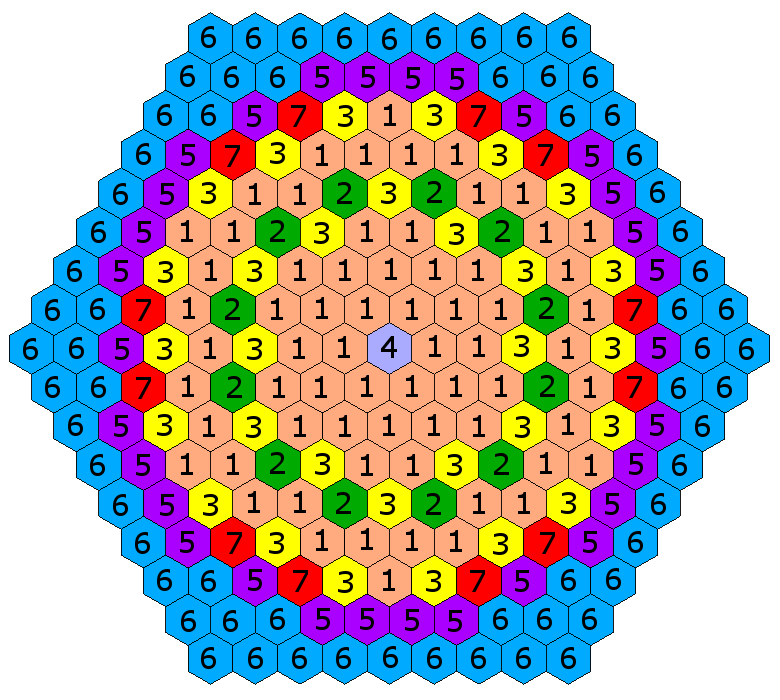
\includegraphics[width=1\linewidth] {1.png}
	\caption{Конечные элементы 1, 2, 3 степени соответственно.}
	\label{fig:1}
  \end{center}
\end{figure} 
Прикладное программное обеспечение написано с использованием библиотеки инженерных и 
научных вычислений FEniCS \cite{fenics}. Для численного решения спектральных задач привлекается библиотека SLEPc \cite{slepc}.


\section{Модельная задача}

Рассматривается тестовая задача для реактора ВВЭР-1000 без отражателя \cite{chao} 
в двумерном приближении ($\Omega$ --- сечение активной зоны реактора). 
Геометрическая модель активной зоны ВВЭР-1000 состоит из набора кассет 
гексагональной формы и представлена на рис.\ref{fig:2}, где цифрами показаны кассеты различных типов.
Размер кассеты «под ключ» равен 23.6 см. 
Диффузионные нейтронно-физические константы при использовании двухгруппового приближения
в общепринятых единицах приведены в табл.\ref{t-1}. 
Используются граничные условия (\ref{3}) при задании $\gamma_g = 0.5, \ g = 1,2$.  
Характеристики запаздывающих нейтронов: используется одна группа запаздывающих нейтронов 
(эффективная доля $\beta_1 = 6.5\cdot10^{-3}$; постоянная распада $\lambda_1 = 0.08$ с$^{-1}$). 
Скорость нейтронов  $v_1 = 1.25 \cdot 10^7$ см/с и  $v_2 = 2.5 \cdot 10^5$ см/с.

\begin{table}[H]
\caption{Диффузионные константы для ВВЭР-1000}
\label{t-1}
\begin{center}
\begin{tabular}{|c|c|c|c|c|c|}
\hline
Материал & 1 & 2 & 3 & 4 & 5\\
\hline
$D_1$ & 1.38320e-0 & 1.38299e-0  & 1.39522e-0  & 1.39446e-0  & 1.39506e-0 \\
$D_2$ & 3.86277e-1 & 3.89403e-1 & 3.86225e-1 & 3.87723e-1 & 3.84492e-1 \\
$\Sigma_1 + \Sigma_{s,1\rightarrow 2}$ & 2.48836e-2 & 2.62865e-2 & 2.45662e-2 & 2.60117e-2 & 2.46141e-2\\
$\Sigma_2$ & 6.73049e-2 & 8.10328e-2 & 8.44801e-1 & 9.89671e-2 & 8.93878e-2\\
$\Sigma_{s,1\rightarrow 2}$ & 1.64977e-2 & 1.47315e-2 & 1.56219e-2 & 1.40185e-2 & 1.54981e-2\\
$\nu\Sigma_{f1}$ & 4.81619e-3 & 4.66953e-3 & 6.04889e-3 & 5.91507e-3 & 6.40256e-3\\
$\nu\Sigma_{f2}$ & 8.46154e-2 & 8.52264e-2 & 1.19428e-1 & 1.20497e-1 & 1.29281e-1\\
\hline
\end{tabular}
\end{center}
\end{table}

\begin{figure}[H]
  \begin{center}
    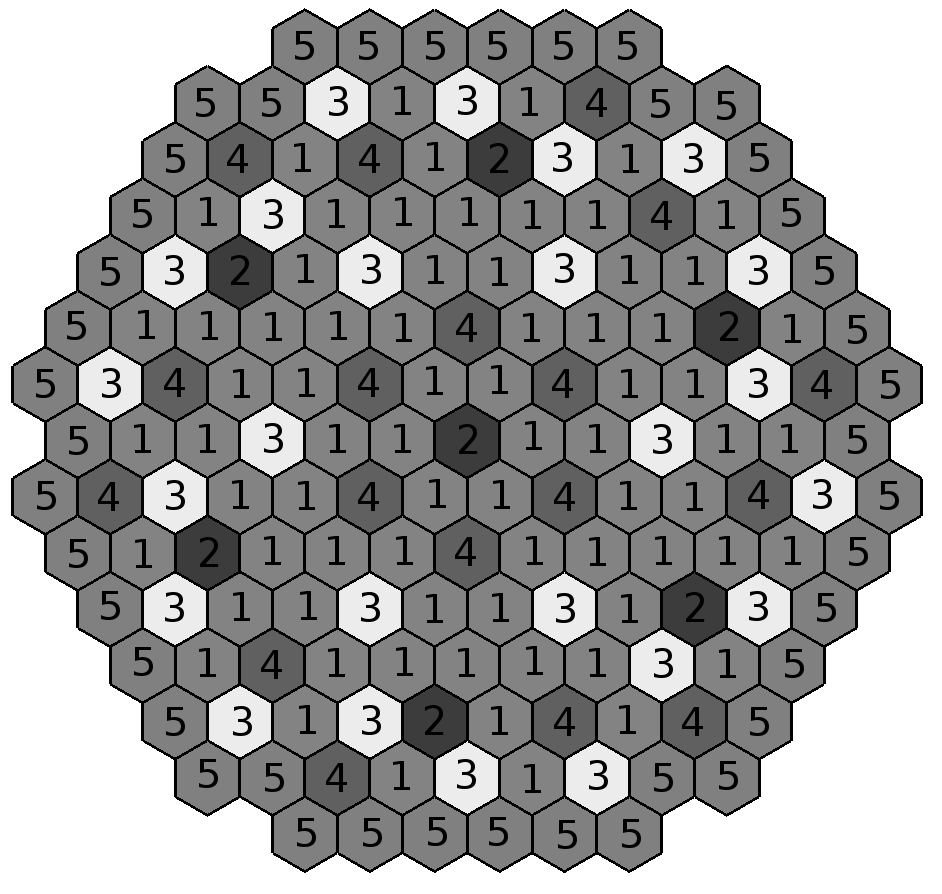
\includegraphics[width=0.75\linewidth] {2.png}
	\caption{Геометрическая модель активной зоны реактор ВВЭР-1000.}
	\label{fig:2}
  \end{center}
\end{figure} 

Для приближенного решение задачи используется регулярные треугольные сетки.
Число треугольников на одну кассету $\kappa$  варьируется от 6 до 96 (рис.\ref{fig:3}). 

\begin{figure}[H]
  \begin{center}
\begin{minipage}{0.30\linewidth}
\center{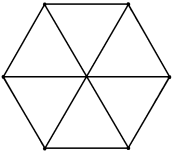
\includegraphics[width=1\linewidth]{3-1.png}}\\
\end{minipage}
\hfill
\begin{minipage}{0.30\linewidth}
\center{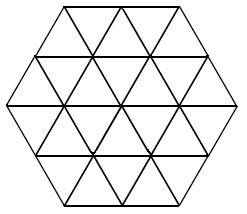
\includegraphics[width=1\linewidth]{3-2.png}}\\
\end{minipage}
\hfill
\begin{minipage}{0.30\linewidth}
\center{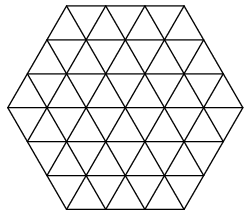
\includegraphics[width=1\linewidth]{3-3.png}}\\
\end{minipage}
\caption{Разбиение кассеты на 6, 24 и 96 конечных элементов.}
\label{fig:3}
  \end{center}
\end{figure}

Задача рассматривается в двухгрупповом приближении с учетом и без учета запаздывающих нейтронов.
Чисто неявная схема (\ref{10}) с учетом запаздывающих нейтронов принимает вид 

\begin{equation}\label{17}
\begin{split}
\frac{1}{\tau v_1} \phi_1^{n+1} &- \nabla \cdot D_1 \nabla \phi_1^{n+1}  + \Sigma_1 \phi_1^{n+1} + \Sigma_{s,1\rightarrow 2} \phi_1^{n+1} - \\  
 &-(1-\beta_1)(\nu \Sigma_{f1} \phi_1^{n+1} + \nu \Sigma_{f2} \phi_2^{n+1}) 
 = \frac{1}{\tau v_1}   \phi_1^{n} + \lambda_1 c_1^{n+1}, \\
\frac{1}{\tau v_2} \phi_2^{n+1} &- \nabla \cdot D_2 \nabla \phi_2^{n+1}  + \Sigma_2 \phi_2^{n+1} - \Sigma_{s,1\rightarrow 2} \phi_1^{n+1}  
 = \frac{1}{\tau v_2}\phi_2^{n}, \\
 c_1^{n+1} &=  e^{-\lambda_1\tau} c_1^n + \tau\beta_1(\nu \Sigma_{f1} \phi_1^{n+1} + \nu \Sigma_{f2} \phi_2^{n+1}).
\end{split}
\end{equation} 
В случае явно-неявной схемы (\ref{12}) имеем:
\begin{equation}\label{18}
\begin{split}
\frac{1}{\tau v_1} \phi_1^{n+1} &- \nabla \cdot D_1 \nabla \phi_1^{n+1} + \Sigma_1 \phi_1^{n+1} + \Sigma_{s,1\rightarrow 2} \phi_1^{n+1}\ = \\ 
&= \frac{1}{\tau v_1}\phi_1^{n} + (1-\beta_1)(\nu \Sigma_{f1} \phi_1^{n} + \nu \Sigma_{f2} \phi_2^{n})+\lambda_1 c_1^{n+1}, \\
\frac{1}{\tau v_2} \phi_2^{n+1} &- \nabla \cdot D_2 \nabla \phi_2^{n+1} + \Sigma_2 \phi_2^{n+1} - \Sigma_{s,1\rightarrow 2} \phi_1^{n+1} = \frac{1}{\tau v_2}\phi_2^{n},\\
c_1^{n+1} &= e^{-\lambda_1\tau} c_1^n + \tau e^{-\lambda_1\tau}\beta_1 (\nu \Sigma_{f1} \phi_1^{n} + \nu \Sigma_{f2} \phi_2^{n})
\end{split}
\end{equation} 
Для начального условия (\ref{8}) рассматриваемой задачи  положим
\[ 
\phi_1^0 = 1, \quad \phi_2^0 = 0.25,
 \quad s_1^0 = \frac{\beta_1}{\lambda_1} (\nu \Sigma_{f1} \phi_1^{0} + \nu \Sigma_{f2} \phi_2^{0}) .
\]

Аналогично формулируются задачи без учета запаздывающий нейтронов. 
Для чисто неявной схемы (\ref{11}) имеем
\begin{equation}\label{19}
\begin{split}
\frac{1}{\tau v_1} \phi_1^{n+1} &- \nabla \cdot D_1 \nabla \phi_1^{n+1} + \Sigma_1 \phi_1^{n+1} + \Sigma_{s,1\rightarrow 2} \phi_1^{n+1} - \\
&- (\nu \Sigma_{f1} \phi_1^{n+1} + \nu \Sigma_{f2} \phi_2^{n+1}) = \frac{1}{\tau v_1}\phi_1^{n}, \\
\frac{1}{\tau v_2} \phi_2^{n+1} &- \nabla \cdot D_2 \nabla \phi_2^{n+1}  + \Sigma_2 \phi_2^{n+1} - \Sigma_{s,1\rightarrow 2} \phi_1^{n+1}  
 = \frac{1}{\tau v_2}\phi_2^{n}.
\end{split}
\end{equation} 
В случае явно-неявной схемы (\ref{13}) имеем
\begin{equation}\label{20}
\begin{split}
\frac{1}{\tau v_1} \phi_1^{n+1} &- \nabla \cdot D_1 \nabla \phi_1^{n+1}  + \Sigma_1 \phi_1^{n+1} + \Sigma_{s,1\rightarrow 2} \phi_1^{n+1}  
 = \frac{1}{\tau v_1} \phi_1^{n} + \\
 &+ (\nu \Sigma_{f1} \phi_1^{n} + \nu \Sigma_{f2} \phi_2^{n}), \\
\frac{1}{\tau v_2} \phi_2^{n+1} &- \nabla \cdot D_2 \nabla \phi_2^{n+1} + \Sigma_2 \phi_2^{n+1} - \Sigma_{s,1\rightarrow 2} \phi_1^{n+1}  
 = \frac{1}{\tau v_2}\phi_2^{n}.
\end{split}
\end{equation} 
Для схемы Кранка-Николсон (\ref{14}) получим
\begin{equation}\label{21}
\begin{split}
\frac{2}{\tau v_1} \phi_1^{n+1} &- \nabla \cdot D_1 \nabla \phi_1^{n+1}  + \Sigma_1 \phi_1^{n+1} + \Sigma_{s,1\rightarrow 2} \phi_1^{n+1}  - (\nu \Sigma_{f1} \phi_1^{n+1} + \nu \Sigma_{f2} \phi_2^{n+1}) = \\
&= \frac{2}{\tau v_1}\phi_1^{n} + \nabla \cdot D_1 \nabla \phi_1^{n}  - \Sigma_1 \phi_1^{n} - \Sigma_{s,1\rightarrow 2} \phi_1^{n}  + (\nu \Sigma_{f1} \phi_1^{n} + \nu \Sigma_{f2} \phi_2^{n}), \\
\frac{2}{\tau v_2} \phi_2^{n+1} &- \nabla \cdot D_2 \nabla \phi_2^{n+1}  + \Sigma_2 \phi_2^{n+1} - \Sigma_{s,1\rightarrow 2} \phi_1^{n+1} = \\
&= \frac{2}{\tau v_2}\phi_2^{n} + \nabla \cdot D_2 \nabla \phi_2^{n}  - \Sigma_2 \phi_2^{n} + \Sigma_{s,1\rightarrow 2} \phi_1^{n}.
\end{split}
\end{equation}
Начальное состояние описывается как и в случае задачи с учетом запаздывающих нейтронов.


Для характеристики динамических процессов в ядерном реакторе, которые описываются задачей Коши 
(\ref{6}),(\ref{7}),(\ref{8}) привлекаются решения некоторых спектральных задач \cite{hetrick1971dynamics,stacey,Bell1970}.
Обычно рассматривается спектральная задача, которая связывается со стационарным состоянием ядерного реактора.
С учетом запаздывающих нейтронов она формулируется в виде
\begin{equation}\label{22}
\begin{split}
(D+S) \bm \varphi  &= \mu  (R \bm \varphi + B \bm s),\\
\Lambda \bm s &= \mu Q \bm \varphi .
\end{split}
\end{equation} 
Аналогично, без учета запаздывающих нейтронов:
\begin{equation}\label{23}
\begin{split}
(D+S) \bm \varphi  &= \mu \widetilde{R} \bm \varphi.\\
\end{split}
\end{equation} 

Это задача (\ref{22}),(\ref{23}) известна как $\lambda$-спектральная задача. 
Для характеристики нейтронного поля привлекается минимальное собственное значение, так что
\[
 k = \frac{1}{\mu^{(1)}}  
\] 
есть эффективный коэффициент размножения.
Значение $k = \mu^{(1)} = 1$ связывается с критическим состоянием реактора, соответствующая
собственная функция $\bm \varphi^{(1)}(\bm x)$ есть стационарное решение уравнения (\ref{5}).
При $k > 1$  говорят о надкритическом состоянии реактора, при $k < 1$  --- о подкритическом состоянии.

Спектральную задачу (\ref{22}),(\ref{23}) нельзя напрямую связать с динамическими процессами в ядерном реакторе.
В лучшем случае мы можем выделить только предельный случай --- стационарное критическое состояние.
Более приемлемая спектральная характеристика для нестационарного уравнения (\ref{5}) связана с $\alpha$-спектральной задачей.
С учетом запаздывающих нейтронов она имеет вид
\begin{equation}\label{24}
\begin{split}
 (D+S - R) \bm \varphi  -  B \bm s & = \mu V \bm \varphi , \\
 \Lambda \bm s - Q \bm \varphi & =  \mu   \bm s .
\end{split} 
\end{equation} 
Без учета запаздывающих нейтронов имеем
\begin{equation}\label{25}
(D + S - \widetilde{R})\bm \varphi  =  \mu V \bm \varphi.
\end{equation} 
Главное собственное значение
\[ 
 \alpha = \mu^{(1)}
\]
называется $\alpha$--собственным значением или  собственным значением периода ядерного реактора \cite{Bell1970}.
С собственным значением $\alpha$ 
можно связать асимптотическое поведение
решения задачи Коши (\ref{6}), (\ref{7}), (\ref{8}) при больших временах. 
На развитой стадии процесса при достаточно больших временах реализуется так называемый регулярный режим \cite{luikov2012analytical,samarskii1996computational}. 
В этом случае в силу быстрого возрастания собственных чисел $\mu^{(i)}$ с номером гармоники $i$ 
влияние высших гармоник практически не проявляется. 
В этом регулярном режиме поведение реактора описывается функцией $e^{-\alpha t} \bm\varphi^{(1)}(\bm x)$, 
то есть поведение решения определяется только первой гармоникой. 
На данной стадии процесса влияние начальных условий играет второстепенную роль.

\section{Результаты расчетов}

Приведем результаты численного решения спектральной задачи (\ref{25}) --- 
без учета запаздывающих нейтронов.
В рамках используемого двухгруппового приближения имеем 
\begin{equation}\label{26}
\begin{split}
 - \nabla \cdot D_1 \nabla \varphi_1 & + \Sigma_1 \varphi_1 + \Sigma_{s,1\rightarrow 2} \varphi_1  
 - (\nu \Sigma_{f1} \varphi_1 + \nu \Sigma_{f2} \varphi_2) = \mu \frac{1}{v_1}   \varphi_1, \\
 - \nabla \cdot D_2 \nabla \varphi_2 & + \Sigma_2 \varphi_2 - \Sigma_{s,1\rightarrow 2} \varphi_1  
 = \mu \frac{1}{v_2}   \varphi_2.
\end{split}
\end{equation} 
Ищется главное собственное значение $\alpha = \mu^{(1)}$ при
\[
\mathrm{Re}  \mu^{(1)} \leq  \mathrm{Re}  \mu^{(2 )} \leq ... \, .
\]

Результаты решения спектральной задачи (\ref{26}) для первых собственных значений $\alpha_i = \mu^{(i)}, \ i = 1,2, ..., 5, \  \mathrm{Re} \mu^{(1)} \leq  \mathrm{Re} \mu^{(2 )} \leq ...$
на разных расчетных сетках при использовании различных
конечно-элементных аппроксимаций показаны в табл.\ref{t-2}. Собственные значения $\alpha_2, \alpha_3$, $\alpha_4, \alpha_5$, $\alpha_9, \alpha_{10}$ являются комплексные с малыми мнимыми частями, собственные значения $\alpha_1, \alpha_6$, $\alpha_7, \alpha_8$ --- действительные. 

\begin{table}[H]
\caption{Собственные значения $\alpha_i = \mu^{(i)}, \ i = 1,2, ..., 5$}
\label{t-2}
\begin{center}
\begin{tabular}{|c|c|c|c|c|}
\hline
$\kappa$ & $p$ & $\alpha_1$ &  $\alpha_2, \alpha_3$ &  $\alpha_4, \alpha_5$ \\ 
\hline
   & 1 & -105.032 & 159.802 $\pm$ 0.025510$i$  & 659.109 $\pm$ 0.034667$i$  \\
6  & 2 & -139.090 & 115.793 $\pm$ 0.029186$i$  & 591.782 $\pm$ 0.034667$i$  \\
   & 3 & -140.223 & 114.035 $\pm$ 0.033814$i$  & 588.762 $\pm$ 0.069025$i$  \\
\hline
   & 1 & -130.422 & 126.984 $\pm$ 0.034409$i$  & 608.734 $\pm$ 0.070724$i$  \\
24 & 2 & -140.187 & 114.089 $\pm$ 0.033512$i$  & 588.849 $\pm$ 0.068555$i$  \\
   & 3 & -140.281 & 113.887 $\pm$ 0.033604$i$  & 588.415 $\pm$ 0.068695$i$  \\
\hline
   & 1 & -137.704 & 117.345 $\pm$ 0.033823$i$  & 593.818 $\pm$ 0.069254$i$  \\
96 & 2 & -140.284 & 113.886 $\pm$ 0.033599$i$  & 588.419 $\pm$ 0.068687$i$  \\
   & 3 & -140.308 & 113.842 $\pm$ 0.033603$i$  & 588.336 $\pm$ 0.068690$i$  \\
\hline
\end{tabular}
\end{center}
\end{table}

Сами собственные значения   $\mathrm{Re} \mu^{(1)} \leq \mathrm{Re}  \mu^{(2)} \leq ...$
хорошо отделены друг от друга. В нашем примере главное собственное значение отрицательно 
и поэтому главная гармоника будет нарастать, а все другие будут затухать. 
Тем самым выражен регулярный режим работы реактора. 
Сама величина $\alpha = \mu^{(1)}$ определяет амплитуду развития нейтронного поля и 
непосредственно связывается с периодом реактора в регулярном режиме.

Собственные функции для главного собственного значения ($i=1$) спектральной задачи (\ref{26})  показаны рис.\ref{fig:4}.
Реальная часть собственных функций $\varphi^{(i)}_1, \ i = 2,3,4,5$ приведена 
на  рис.\ref{fig:5}. Мнимая часть этих собственных функций показана  на  рис.\ref{fig:6}.


\begin{figure}[H]
  \begin{center}
\begin{minipage}{0.49\linewidth}
\center{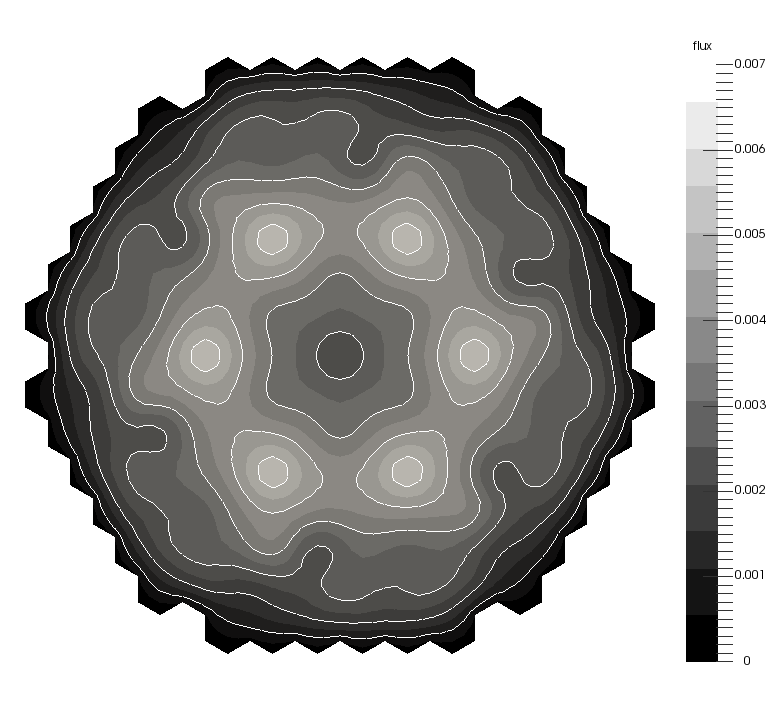
\includegraphics[width=1\linewidth]{4-1.png}} \\
\end{minipage}
\hfill
\begin{minipage}{0.49\linewidth}
\center{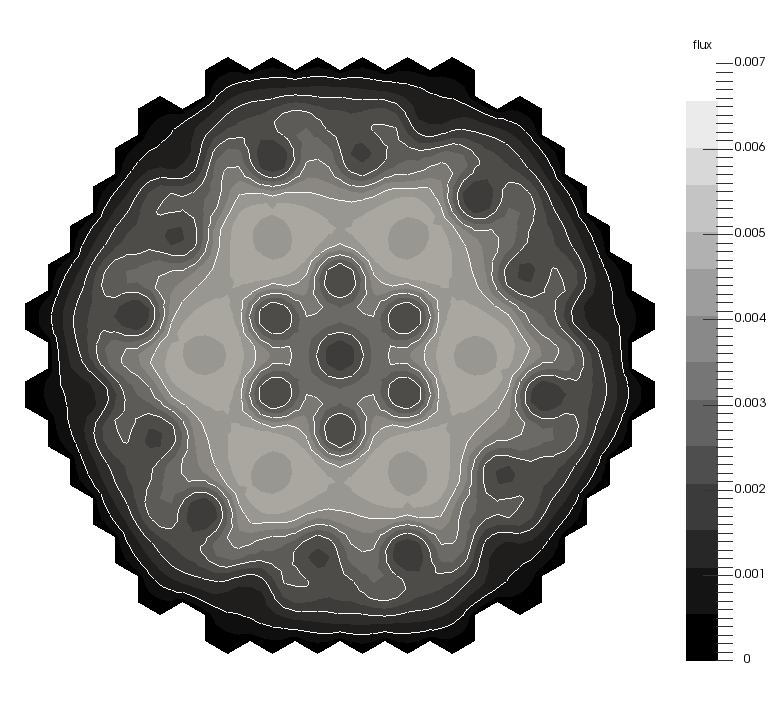
\includegraphics[width=1\linewidth]{4-2.png}} \\
\end{minipage}
\caption{Собственные функции $\varphi^{(1)}_1$ (слева) и $\varphi^{(1)}_2$ (справа).}
\label{fig:4}
  \end{center}
\end{figure}

\begin{figure}[H]
  \begin{center}
\begin{minipage}{0.49\linewidth}
\center{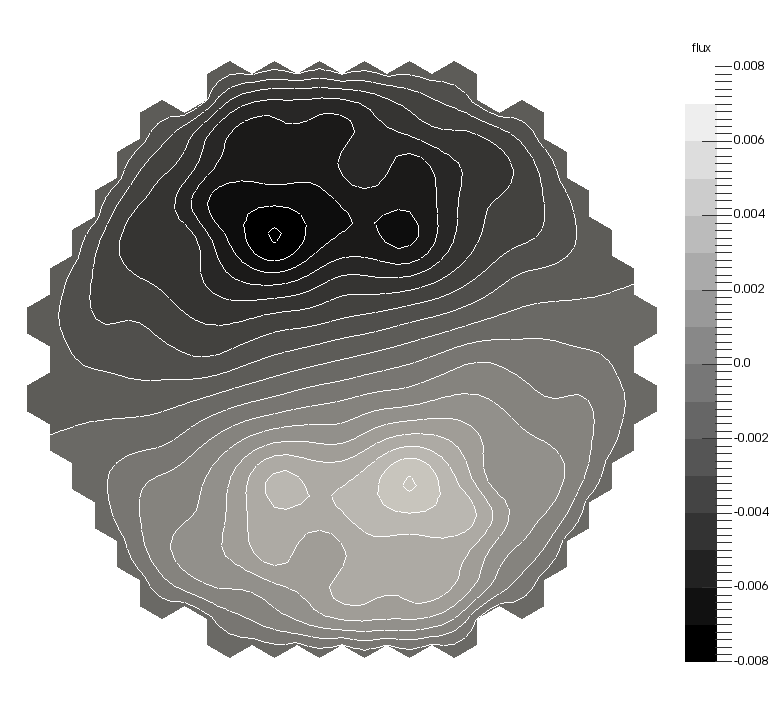
\includegraphics[width=1\linewidth]{5-1.png}} \\
\end{minipage}
\hfill
\begin{minipage}{0.49\linewidth}
\center{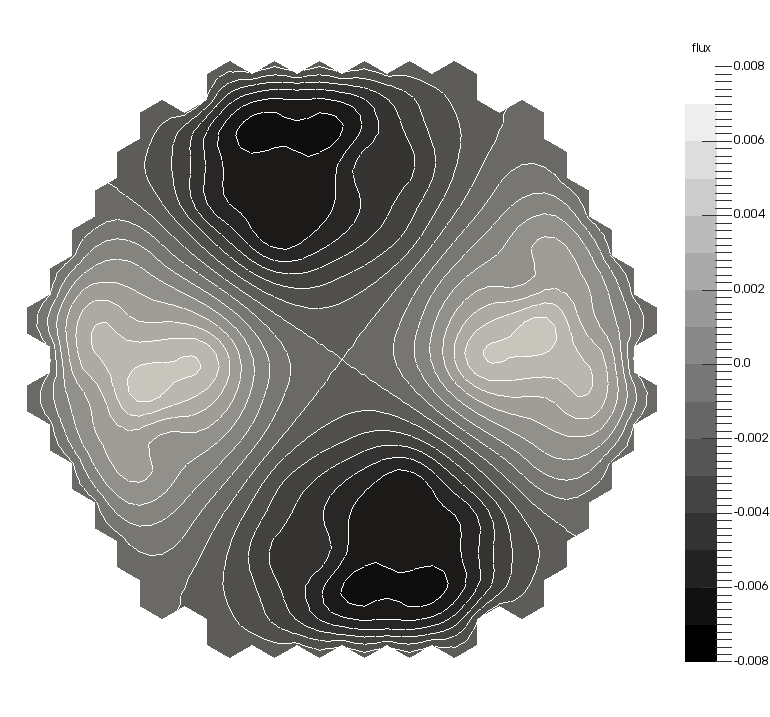
\includegraphics[width=1\linewidth]{5-2.png}} \\
\end{minipage}
\caption{Реальная часть собственных функций $\varphi^{(2)}_1, \ \varphi^{(3)}_1$ (слева) и $\varphi^{(4)}_1, \ \varphi^{(5)}_1$ (справа).}
\label{fig:5}
  \end{center}
\end{figure}

\begin{figure}[H]
  \begin{center}
\begin{minipage}{0.49\linewidth}
\center{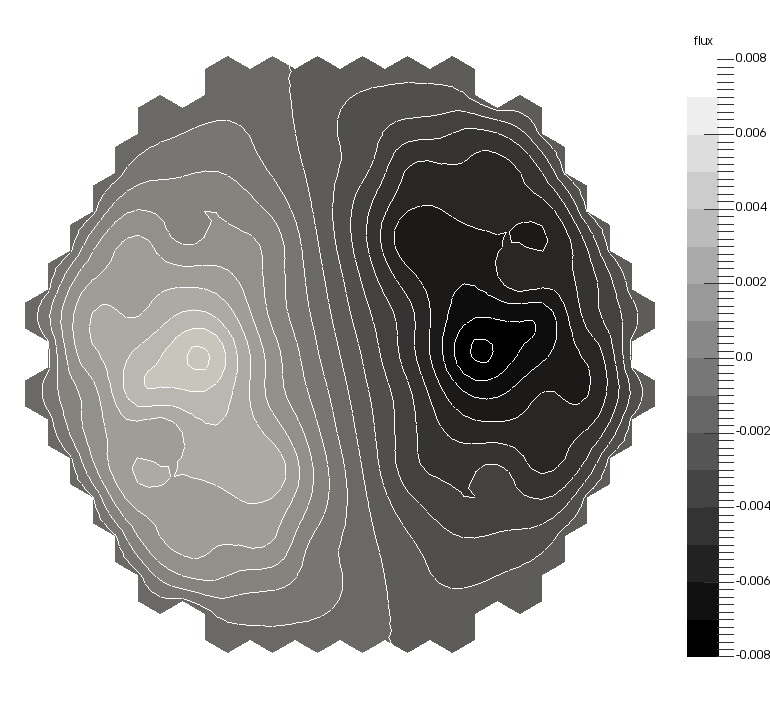
\includegraphics[width=1\linewidth]{6-1.png}} \\
\end{minipage}
\hfill
\begin{minipage}{0.49\linewidth}
\center{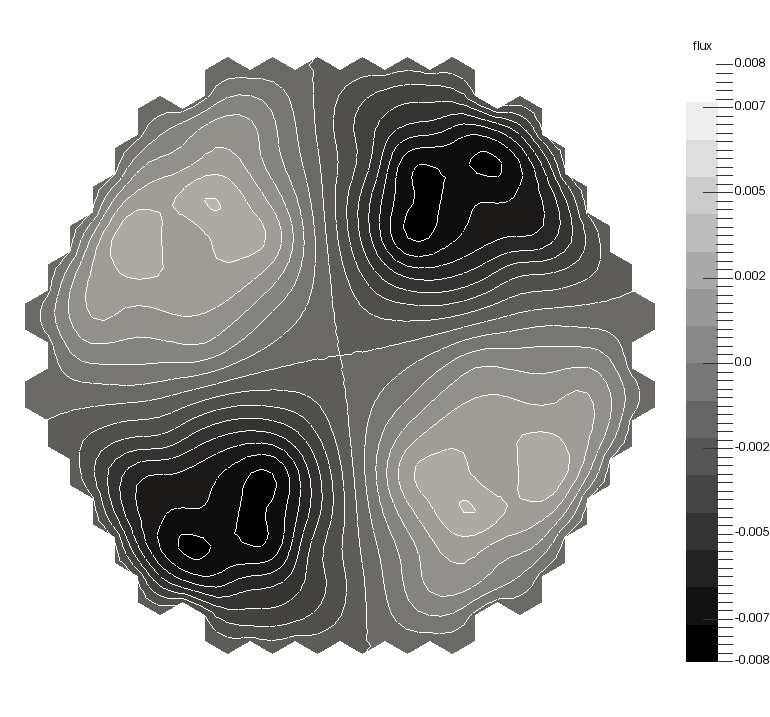
\includegraphics[width=1\linewidth]{6-2.png}} \\
\end{minipage}
\caption{Мнимая часть собственных функций $\varphi^{(2)}_1, \ - \varphi^{(3)}_1$ (слева) и $\varphi^{(4)}_1, \ - \varphi^{(5)}_1$ (справа).}
\label{fig:6}
  \end{center}
\end{figure}

Приведем результаты численного решения спектральной задачи (\ref{24}) с учетом запаздывающих нейтронов.
В рамках используемого двухгруппового приближения имеем 
\begin{equation}\label{27}
\begin{split}
 - \nabla \cdot D_1 \nabla \varphi_1  + \Sigma_1 \varphi_1 + \Sigma_{s,1\rightarrow 2} \varphi_1  
& - (\nu \Sigma_{f1} \varphi_1 + \nu \Sigma_{f2} \varphi_2) - \lambda_1 s_1 = \mu \frac{1}{v_1}   \varphi_1, \\
 - \nabla \cdot D_2 \nabla \varphi_2  + \Sigma_2 \varphi_2 & - \Sigma_{s,1\rightarrow 2} \varphi_1  
 = \mu \frac{1}{v_2}   \varphi_2,\\
\lambda_1 s_1 - \beta_1(\nu \Sigma_{f1} \varphi_1 &+ \nu \Sigma_{f2} \varphi_2) = \mu s_1. 
\end{split}
\end{equation} 
Ищется главное собственное значение $\alpha = \mu^{(1)}$, причем
$\mathrm{Re} \mu^{(1)} \leq \mathrm{Re}  \mu^{(2)} \leq ... \,$.

Результаты решения спектральной задачи (\ref{27}) для первых собственных
значений $\alpha_i = \mu^{(i)}, \ i = 1,2, ..., 5$
на разных расчетных сетках при использовании различных
конечно-элементных аппроксимаций показаны в табл.\ref{t-3}. Как и в задаче
без учета запаздывающих нейтронов собственные значения $\alpha_2, \alpha_3$, $\alpha_4, \alpha_5$, $\alpha_9, \alpha_{10}$ 
для спектральной задачи (\ref{27}) являются комплексные с малыми мнимыми частями, собственные значения $\alpha_1, \alpha_6$, $\alpha_7, \alpha_8$ --- действительные.

\begin{table}[H]
\caption{Собственные значения $\alpha_i = \mu^{(i)}, \ i = 1,2, ..., 5$}
\label{t-3}
\begin{center}
\begin{tabular}{|c|c|c|c|c|}
\hline
$\kappa$ & $p$ & $\alpha_1$ &  $\alpha_2, \alpha_3$ &  $\alpha_4, \alpha_5$ \\ 
\hline
   & 1 & -0.22557 & 0.04241 $\pm$ 3.08808e-06$i$  & 0.06588 $\pm$ 4.80448e-07$i$  \\
6  & 2 & -2.10154 & 0.03592 $\pm$ 4.96474e-06$i$  & 0.06452 $\pm$ 1.21320e-06$i$  \\
   & 3 & -2.47975 & 0.03561 $\pm$ 5.83719e-06$i$  &  0.06445 $\pm$ 1.41869e-06$i$  \\
\hline
   & 1 & -0.82680 & 0.03777 $\pm$ 5.37884e-06$i$  & 0.06489 $\pm$ 1.37315e-06$i$  \\
24 & 2 & -2.46601 & 0.03562 $\pm$ 5.78277e-06$i$  & 0.06445 $\pm$ 1.40897e-06$i$  \\
   & 3 & -2.50294 & 0.03559 $\pm$ 5.80783e-06$i$  & 0.06444 $\pm$ 1.41341e-06$i$  \\
\hline
   & 1 & -1.74998 & 0.03619 $\pm$ 5.69002e-06$i$  & 0.06456 $\pm$ 1.40299e-06$i$  \\
96 & 2 & -2.50375 & 0.03559 $\pm$ 5.80693e-06$i$  & 0.06444 $\pm$ 1.41324e-06$i$  \\
   & 3 & -2.51280 & 0.03558 $\pm$ 5.80954e-06$i$  & 0.06444 $\pm$ 1.41362e-06$i$  \\
\hline

\end{tabular}
\end{center}
\end{table}

Собственные функции для главного собственного значения ($i=1$) спектральной задачи (\ref{27})  показаны рис.\ref{fig:7}. 
Реальная часть собственных функций $\varphi^{(i)}_1, \ i = 2,3,4,5$ приведена на  рис.\ref{fig:8}. Мнимая часть этих собственных функций показана  на  рис.\ref{fig:9}.
Снова главное собственное значение
отрицательно и поэтому главная гармоника
будет нарастать, а все другие будут затухать. Тем самым мы можем наблюдать регулярный режим работы реактора. 

\begin{figure}[H]
  \begin{center}
\begin{minipage}{0.4\linewidth}
\center{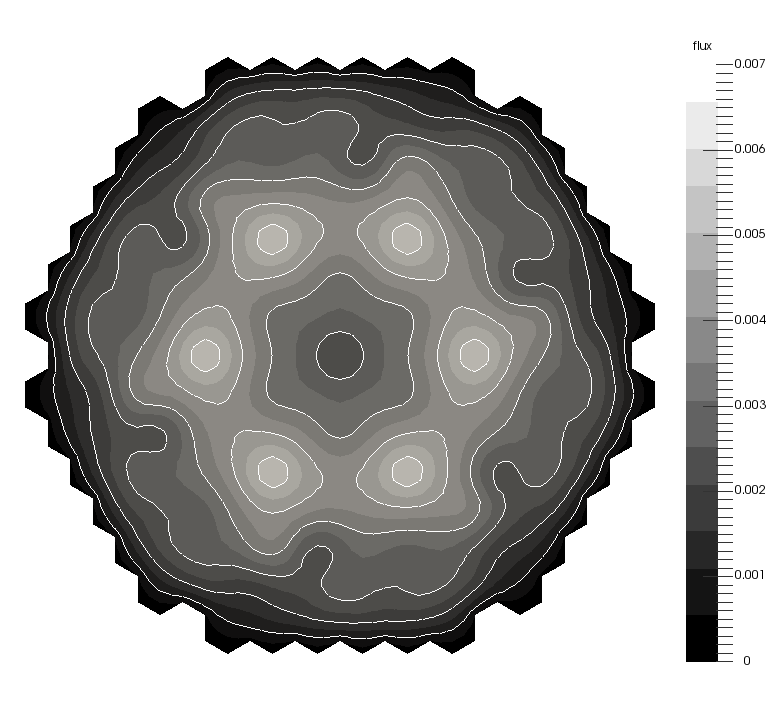
\includegraphics[width=1\linewidth]{7-1.png}} \\
\end{minipage}
\hfill
\begin{minipage}{0.4\linewidth}
\center{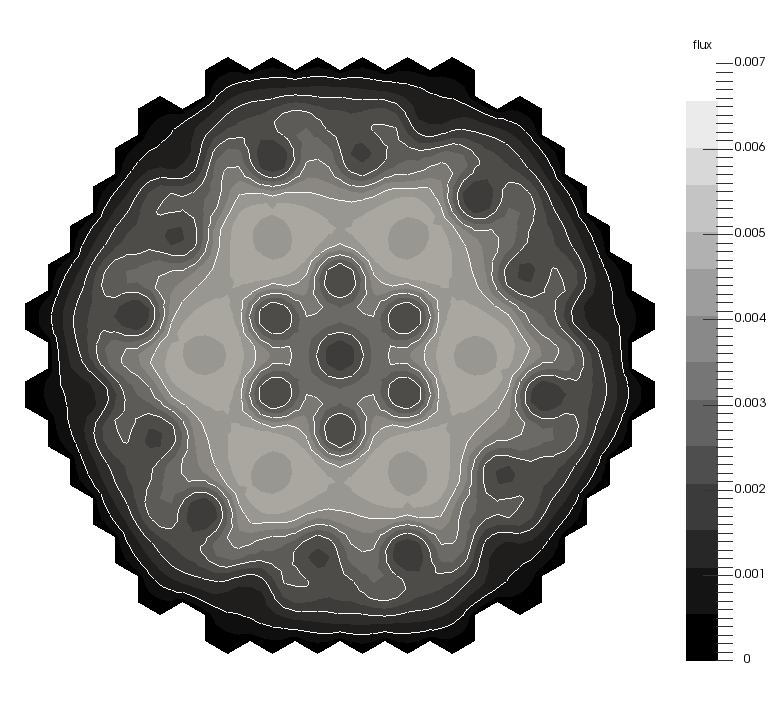
\includegraphics[width=1\linewidth]{7-2.png}} \\
\end{minipage}
\caption{Собственные функции $\varphi^{(1)}_1$ (слева) и $\varphi^{(1)}_2$ (справа).}
\label{fig:7}
  \end{center}
\end{figure}

\begin{figure}[H]
  \begin{center}
\begin{minipage}{0.4\linewidth}
\center{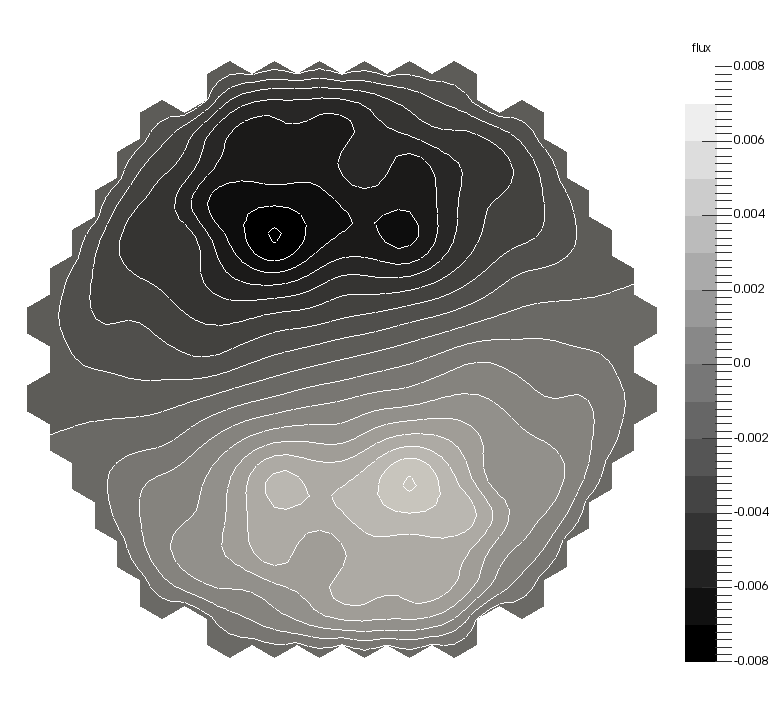
\includegraphics[width=1\linewidth]{8-1.png}} \\
\end{minipage}
\hfill
\begin{minipage}{0.4\linewidth}
\center{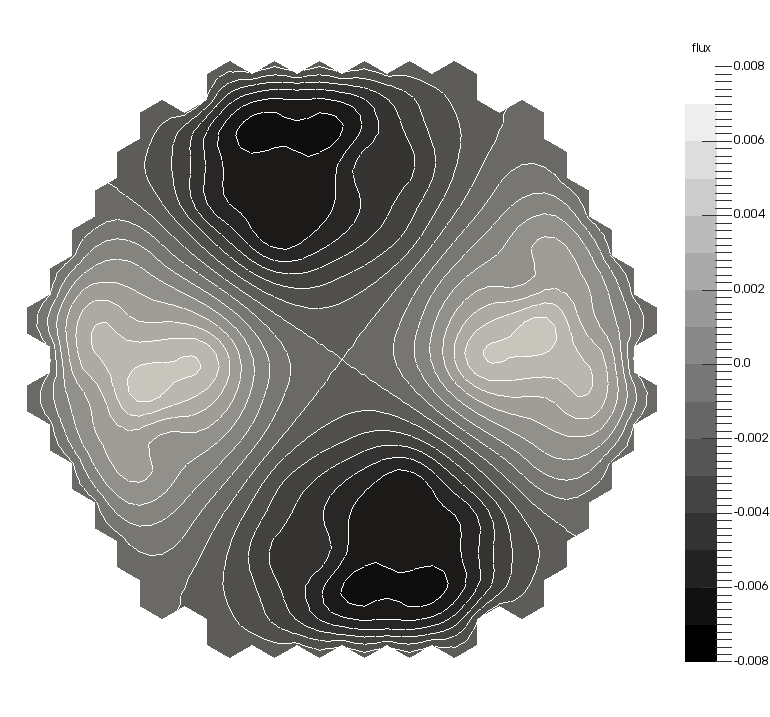
\includegraphics[width=1\linewidth]{8-2.png}} \\
\end{minipage}
\caption{Реальная часть собственных функций $\varphi^{(2)}_1, \ \varphi^{(3)}_1$ (слева) и $\varphi^{(4)}_1, \ \varphi^{(5)}_1$ (справа).}
\label{fig:8}
  \end{center}
\end{figure}

\begin{figure}[H]
  \begin{center}
\begin{minipage}{0.4\linewidth}
\center{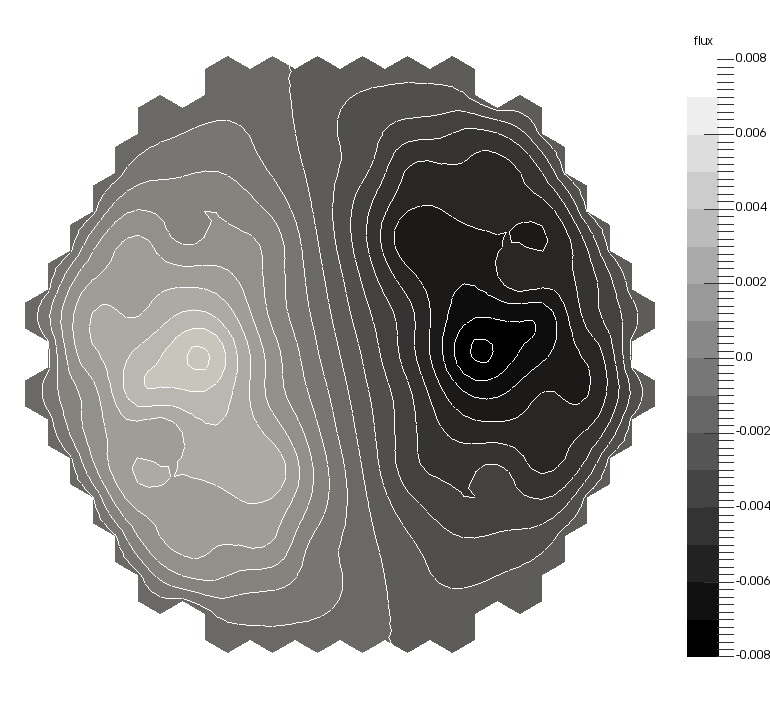
\includegraphics[width=1\linewidth]{9-1.png}} \\
\end{minipage}
\hfill
\begin{minipage}{0.4\linewidth}
\center{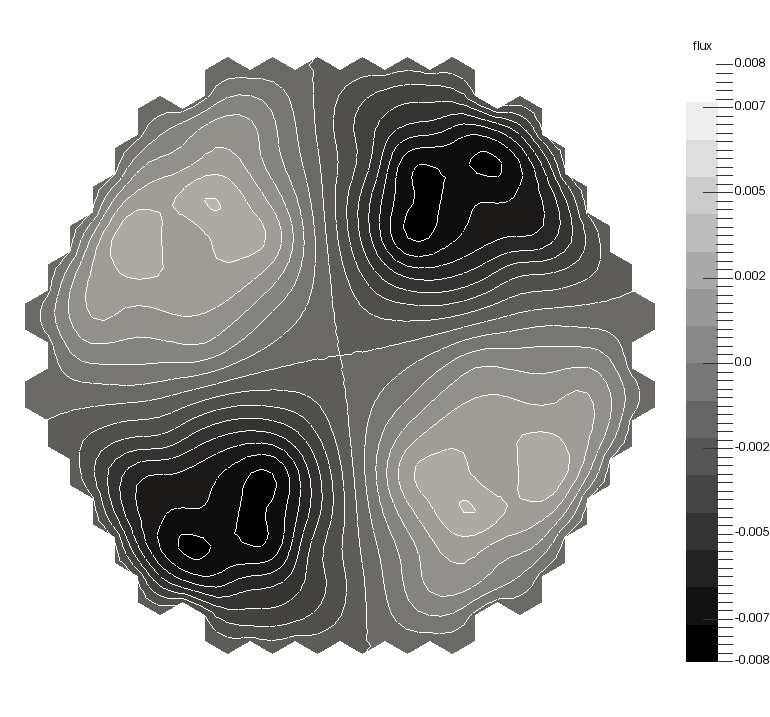
\includegraphics[width=1\linewidth]{9-2.png}} \\
\end{minipage}
\caption{Мнимая часть собственных функций $\varphi^{(2)}_1, \ - \varphi^{(3)}_1$ (слева) и $\varphi^{(4)}_1, \ - \varphi^{(5)}_1$ (справа).}
\label{fig:9}
  \end{center}
\end{figure}

Нестационарные задачи численно решаются при $k=24$ и $p=2$.
Выход на регулярный режим будем контролировать с помощью оценки близости отнормированного решения нестационарной задачи и главной собственной функции
$\bm \varphi = \bm \varphi^{(1)}$. Для первой группы положим
\[
\begin{split}
\eta(t) = \norm{\overline{\phi}_1(\bm x,t)-\overline{\varphi}_1(\bm x,t)}, \quad
\overline{\phi}_1(\bm x,t) = \frac{\phi_1(\bm x,t)}{\norm{\phi_1(\bm x,t)}}, \quad \overline{\varphi}_1(\bm x,t) = \frac{\varphi_1^{(1)}(\bm x,t)}{\norm{\varphi_1^{(1)}(\bm x,t)}}.
\end{split}
\]
Установление темпа динамического развития оценивается величиной
\[
\theta(t) = \frac{1}{\sqrt{2} \norm{\alpha}} \left ( 
\norm{\frac{1}{\phi_1(\bm x,t)}\frac{\partial\phi_1(\bm x,t)}{\partial t} - \alpha}^2 +
\norm{\frac{1}{\phi_2(\bm x,t)}\frac{\partial\phi_2(\bm x,t)}{\partial t} - \alpha}^2 \right )^{1/2} .
\]

При численном решении нестационарной задачи без учета запаздывающих нейтронов
возьмем $T=5\cdot 10^{-3}$. Будем варьировать шаг по времени: положим $\tau=5\cdot 10^{-5}, 1\cdot 10^{-4}, 2\cdot 10^{-4}, 4\cdot 10^{-4}$ в случае чисто неявной схемы 
(\ref{19}) и схемы Кранка-Николсон (\ref{21}) и  $\tau=1.25\cdot 10^{-5}, 2.5\cdot 10^{-5},5\cdot 10^{-5}, 1\cdot 10^{-4}$ в случае явно-неявной схемы (\ref{20}). 
Реперным решением ($ref$) для всех случаев будет приближенное решение при 
использовании чисто неявной схеме при $\tau = 1 \cdot 10^{-5}$.

Зависимости $\eta(t)$ и $\theta(t)$ от используемого шага по времени приведена на рис.\ref{fig:10} для чисто неявной схемы и на рис.\ref{fig:11} для явно-неявной схемы. На рис.\ref{fig:12} показаны зависимости $\eta(t)$ и $\theta(t)$ для схемы Кранка-Николсон. Чисто неявная схема (\ref{11}) имеет существенно более высокую точность, чем явно-неявная схема (\ref{13}). Как и ожидалось, схема Кранка-Николсон практически непригодна для
моделирования регулярного режима в силу того, что она имеет плохие свойства асимптотической устойчивости.

Далее на рис.\ref{fig:13},\ref{fig:14} показаны отнормированые реперные решения $\overline{\phi}_1$ и $\overline{\phi}_2$ на моменты времени $t=0.0001, 0.0004, 0.0016$ и $0.005$ секунд, которые иллюстрируют выход на регулярный режим.  

\begin{figure}[H]
  \begin{center}
\begin{minipage}{0.49\linewidth}
\center{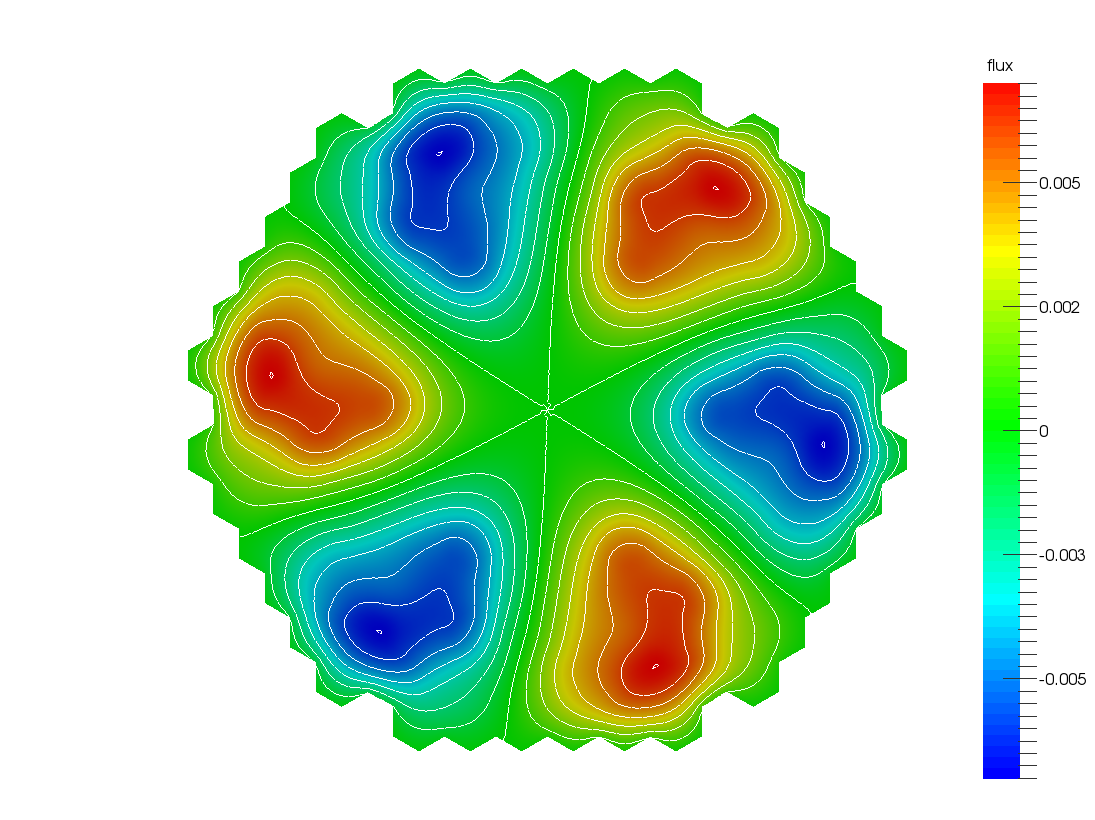
\includegraphics[width=1\linewidth]{10-1.png}} \\
\end{minipage}
\hfill
\begin{minipage}{0.49\linewidth}
\center{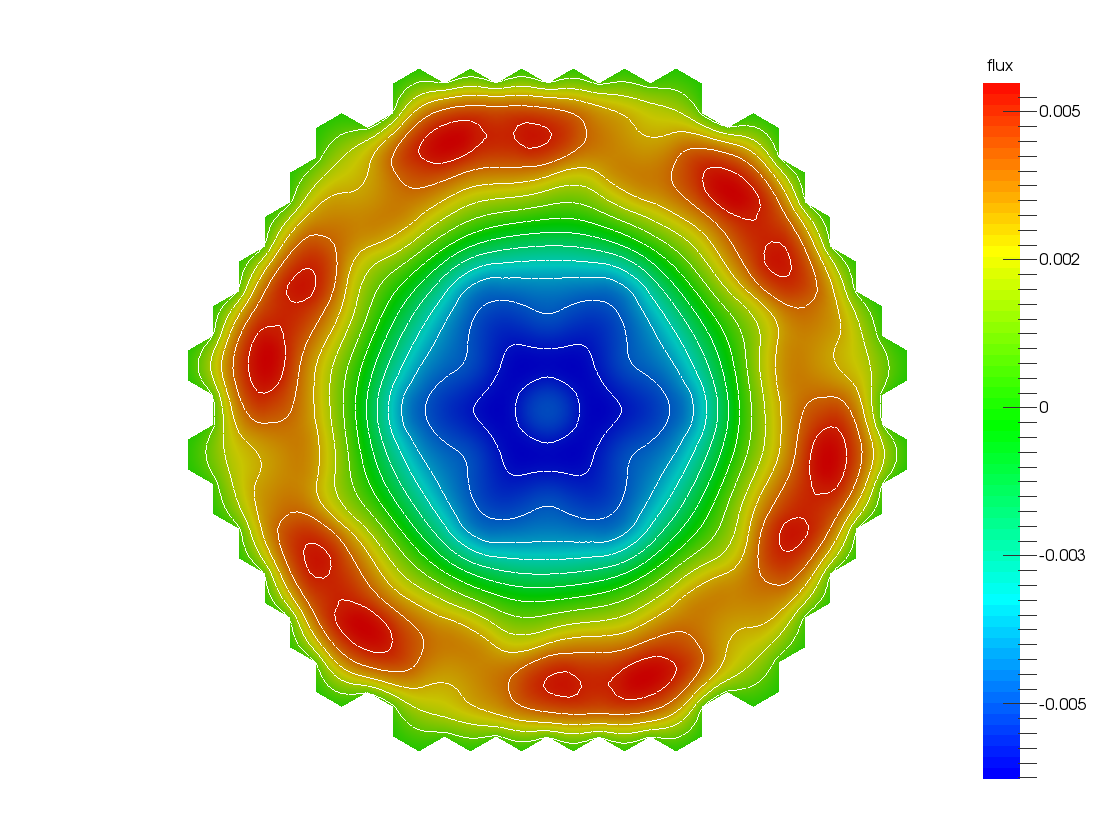
\includegraphics[width=1\linewidth]{10-2.png}} \\
\end{minipage}
\caption{Чисто неявная схема (\ref{19}).}
\label{fig:10}
  \end{center}
\end{figure}


\begin{figure}[H]
  \begin{center}
\begin{minipage}{0.49\linewidth}
\center{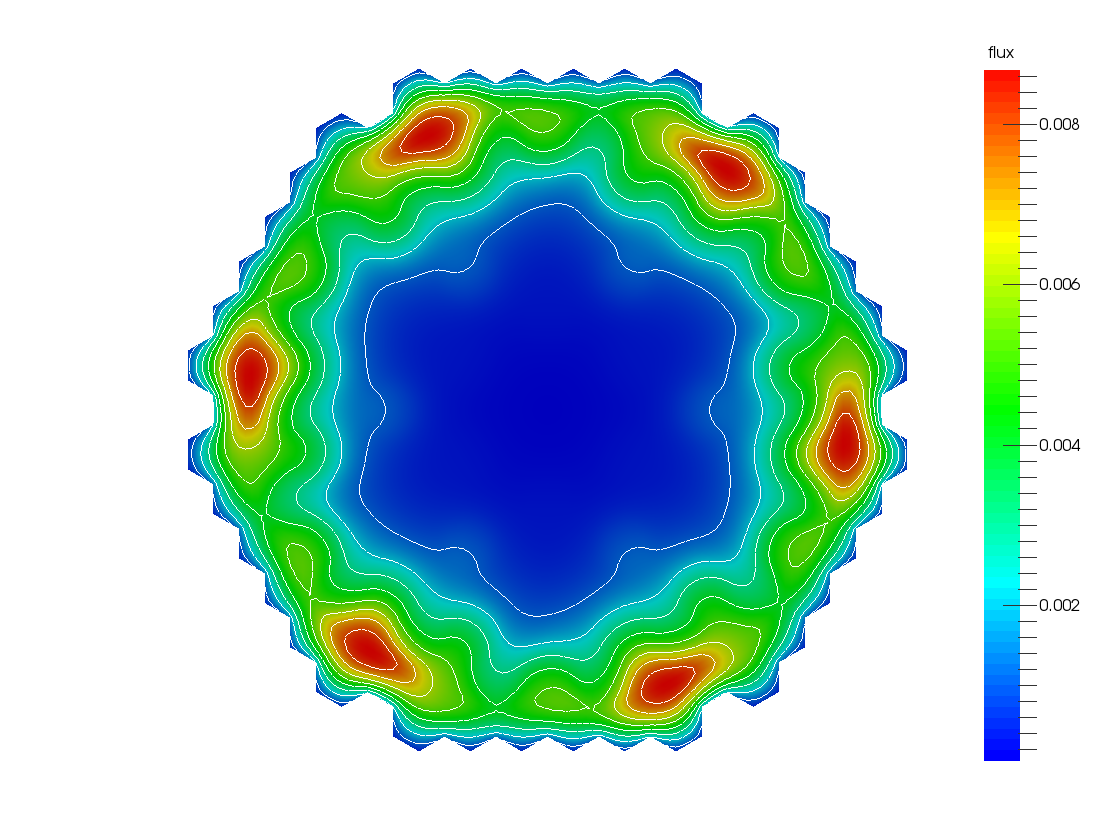
\includegraphics[width=1\linewidth]{11-1.png}} \\
\end{minipage}
\hfill
\begin{minipage}{0.49\linewidth}
\center{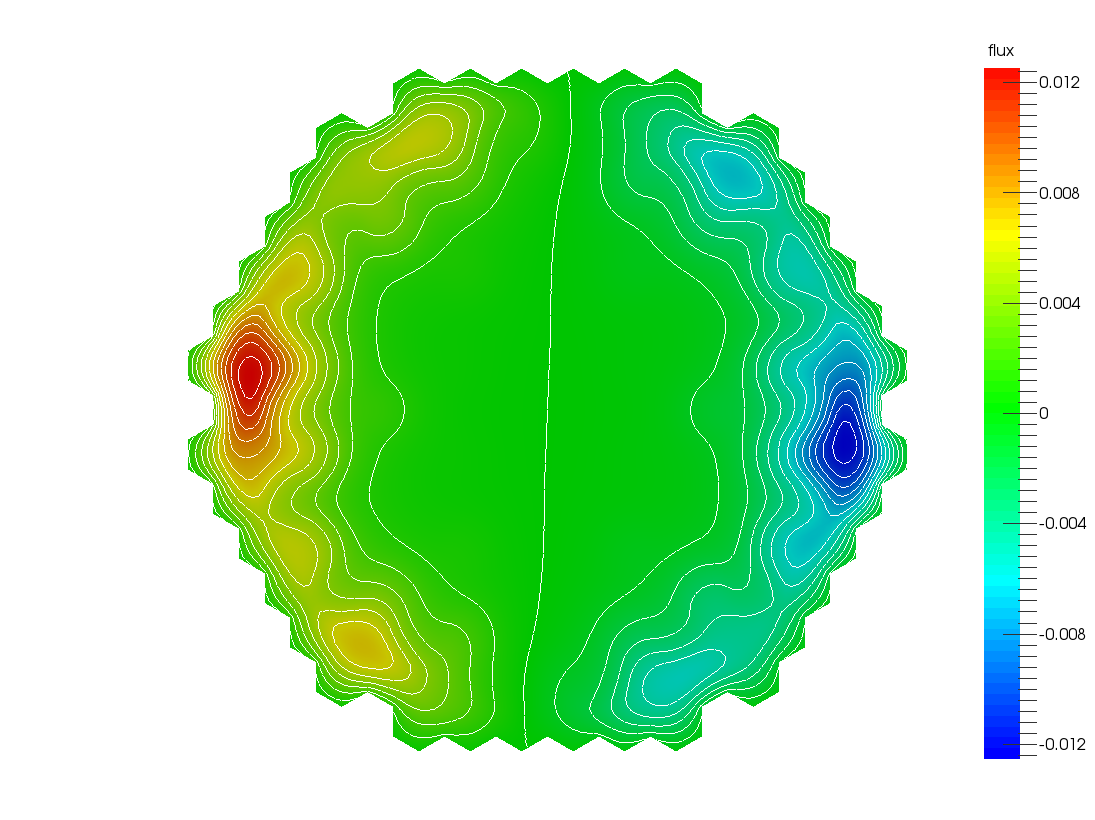
\includegraphics[width=1\linewidth]{11-2.png}} \\
\end{minipage}
\caption{Явно-неявная схема (\ref{21}).}
\label{fig:11}
  \end{center}
\end{figure}


\begin{figure}[H]
  \begin{center}
\begin{minipage}{0.49\linewidth}
\center{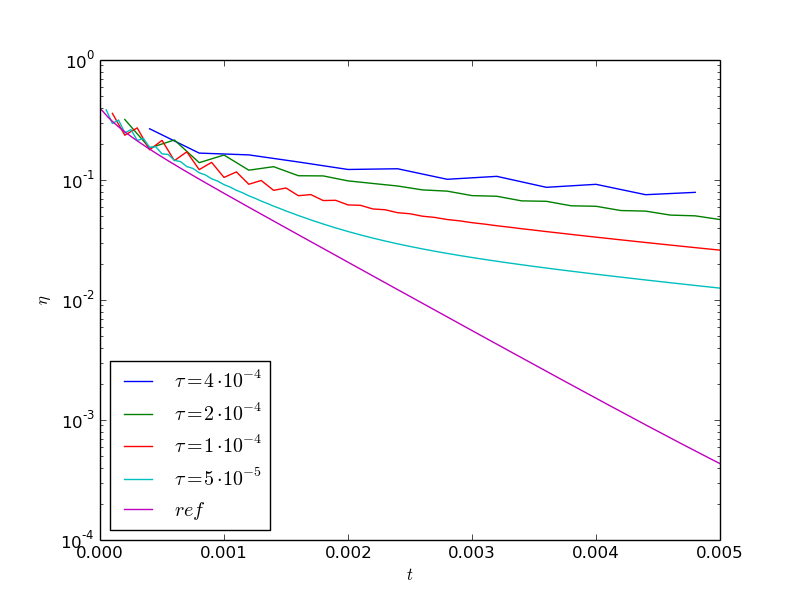
\includegraphics[width=1\linewidth]{12-1.png}} \\
\end{minipage}
\hfill
\begin{minipage}{0.49\linewidth}
\center{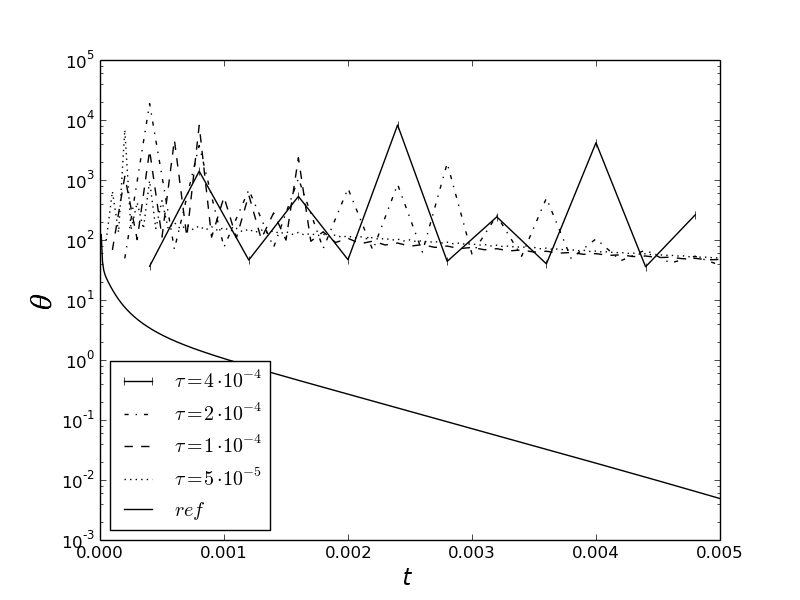
\includegraphics[width=1\linewidth]{12-2.png}} \\
\end{minipage}
\caption{Схема Кранка-Николсон (\ref{20}).}
\label{fig:12}
  \end{center}
\end{figure}

\begin{figure}[H]
\begin{center}
\begin{minipage}{0.49\linewidth}
\center{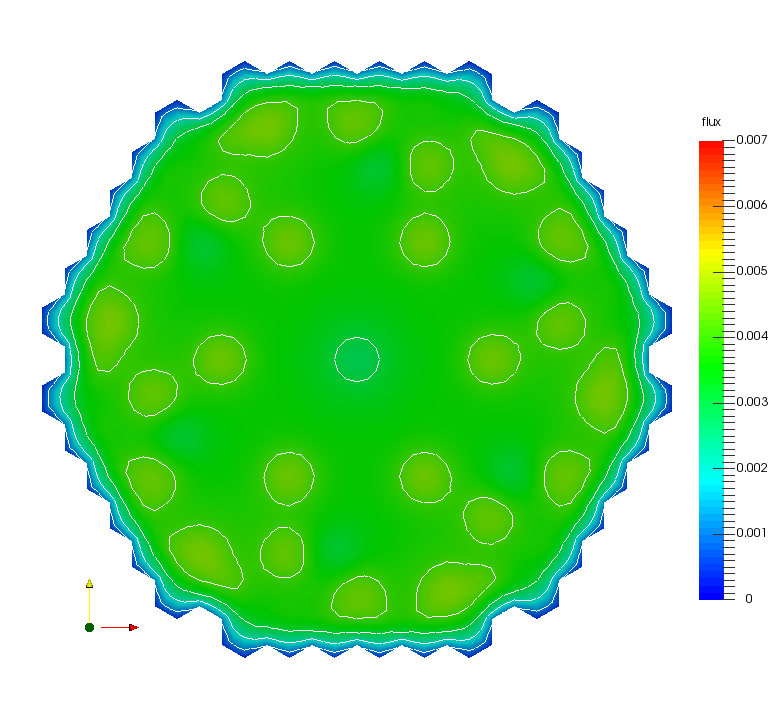
\includegraphics[width=0.9\linewidth]{13-1.png}  $t=0.0001$} \\
\end{minipage}
\hfill
\begin{minipage}{0.49\linewidth}
\center{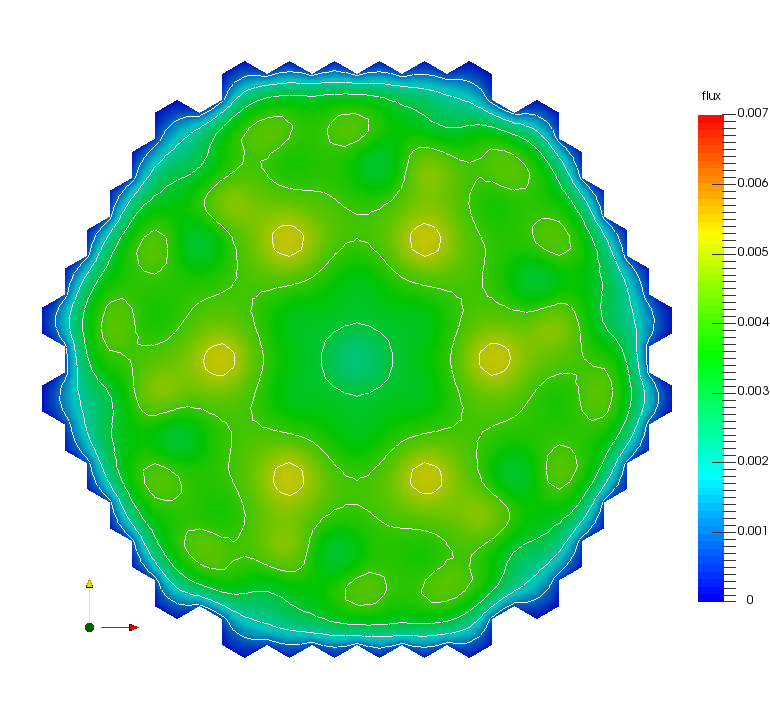
\includegraphics[width=0.9\linewidth]{13-2.png}  $t=0.0004$} \\
\end{minipage}
\hfill
\begin{minipage}{0.49\linewidth}
\center{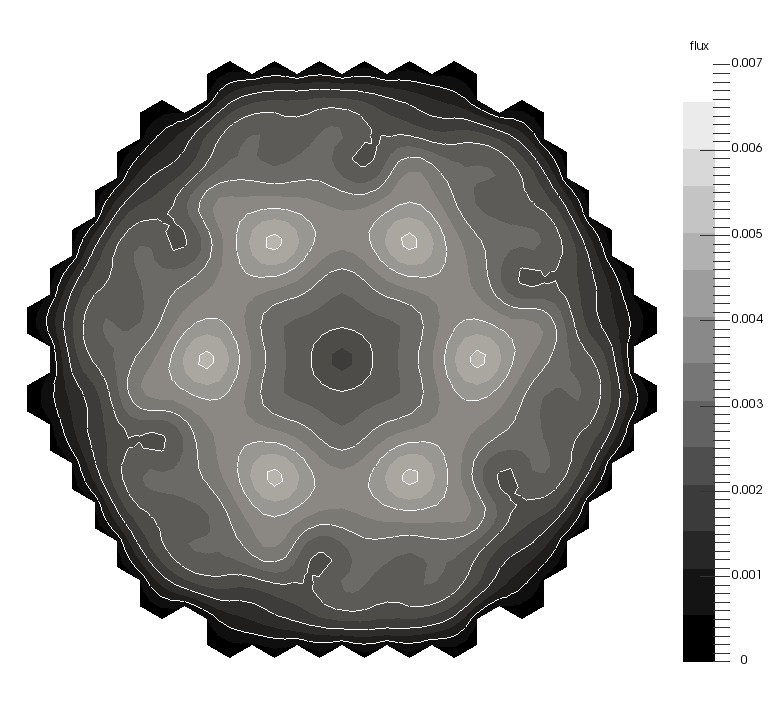
\includegraphics[width=0.9\linewidth]{13-3.png}  $t=0.0016$} \\
\end{minipage}
\hfill
\begin{minipage}{0.49\linewidth}
\center{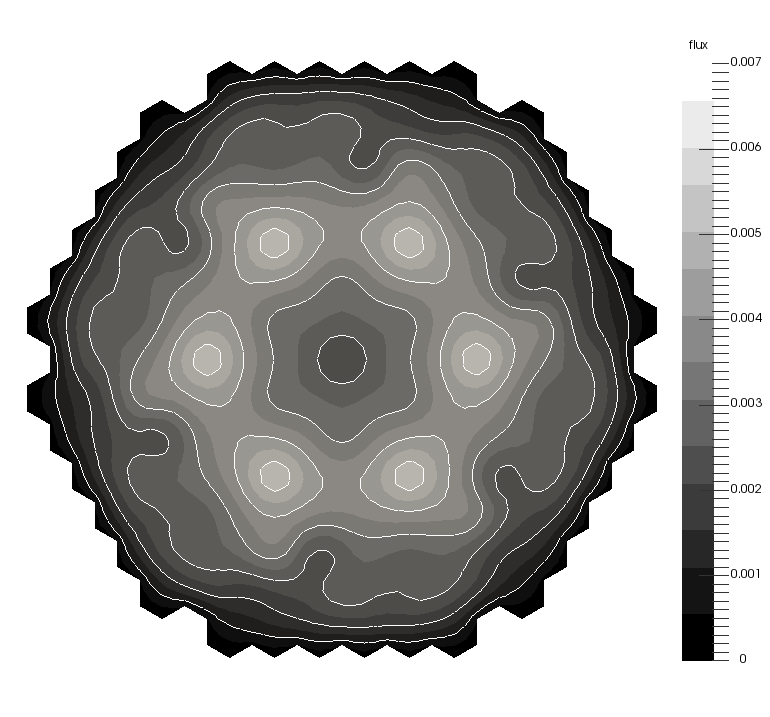
\includegraphics[width=0.9\linewidth]{13-4.png}  $t=0.005$} \\
\end{minipage}
\caption{Эволюция $\phi_1(t)$.}
\label{fig:13}
  \end{center}
\end{figure}

\begin{figure}[H]
\begin{center}
\begin{minipage}{0.49\linewidth}
\center{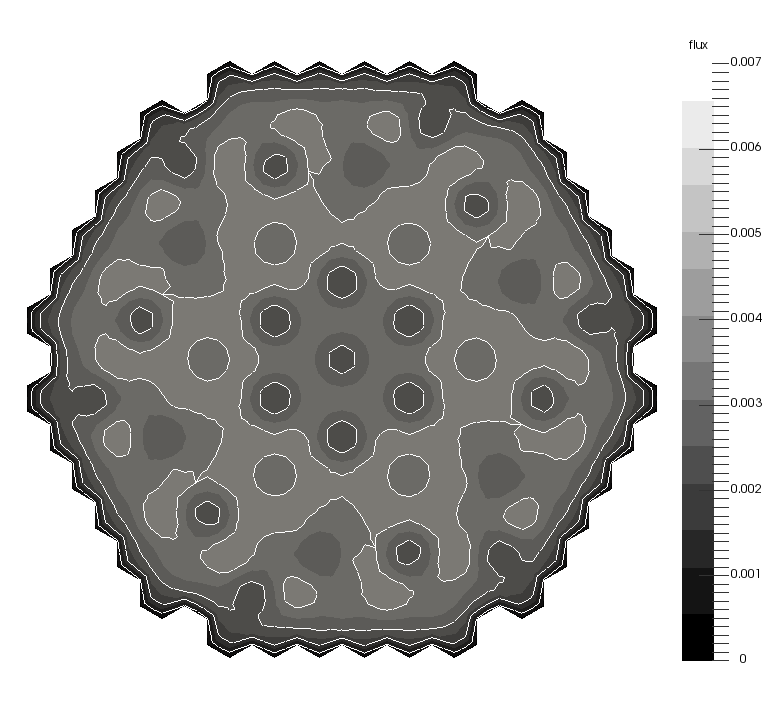
\includegraphics[width=0.9\linewidth]{14-1.png}  $t=0.0001$} \\
\end{minipage}
\hfill
\begin{minipage}{0.49\linewidth}
\center{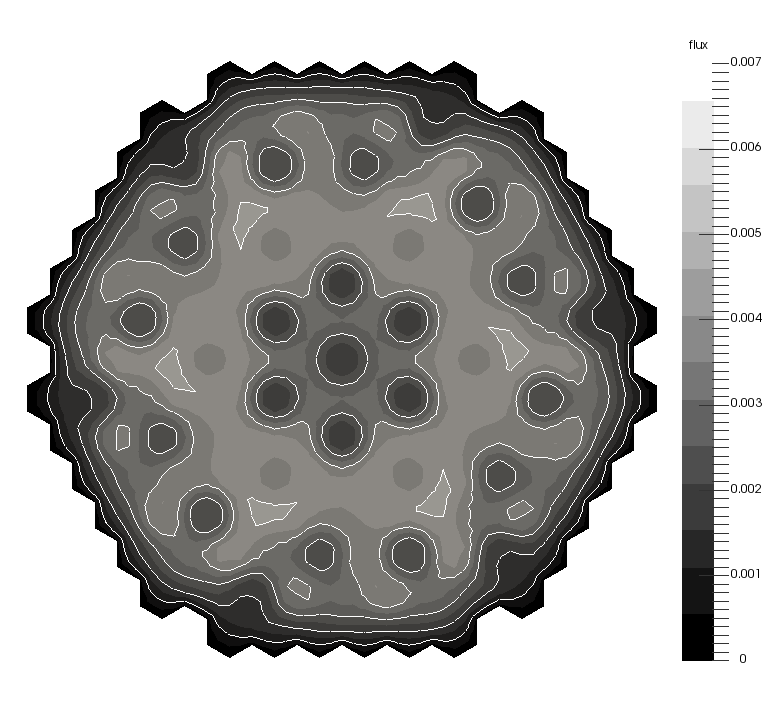
\includegraphics[width=0.9\linewidth]{14-2.png}  $t=0.0004$} \\
\end{minipage}
\hfill
\begin{minipage}{0.49\linewidth}
\center{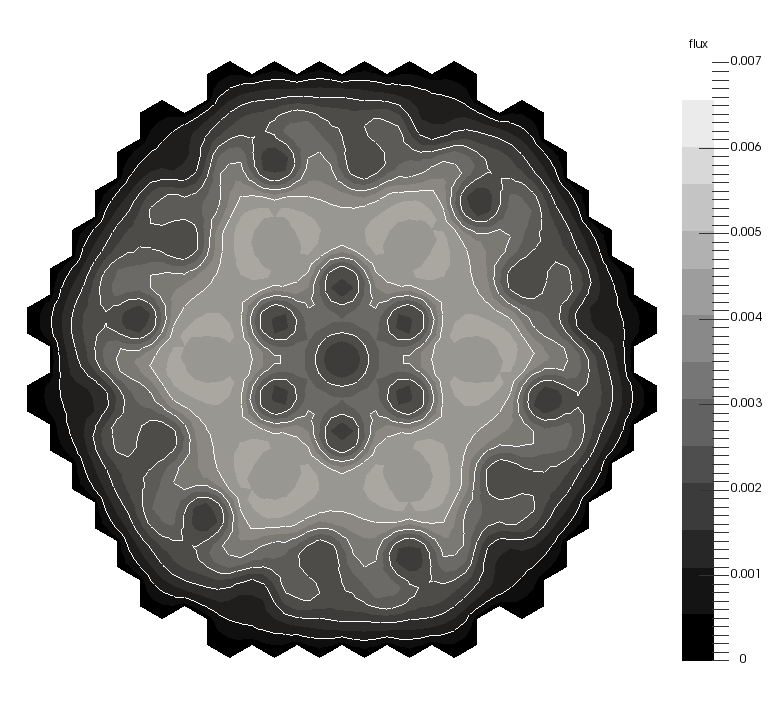
\includegraphics[width=0.9\linewidth]{14-3.png}  $t=0.0016$} \\
\end{minipage}
\hfill
\begin{minipage}{0.49\linewidth}
\center{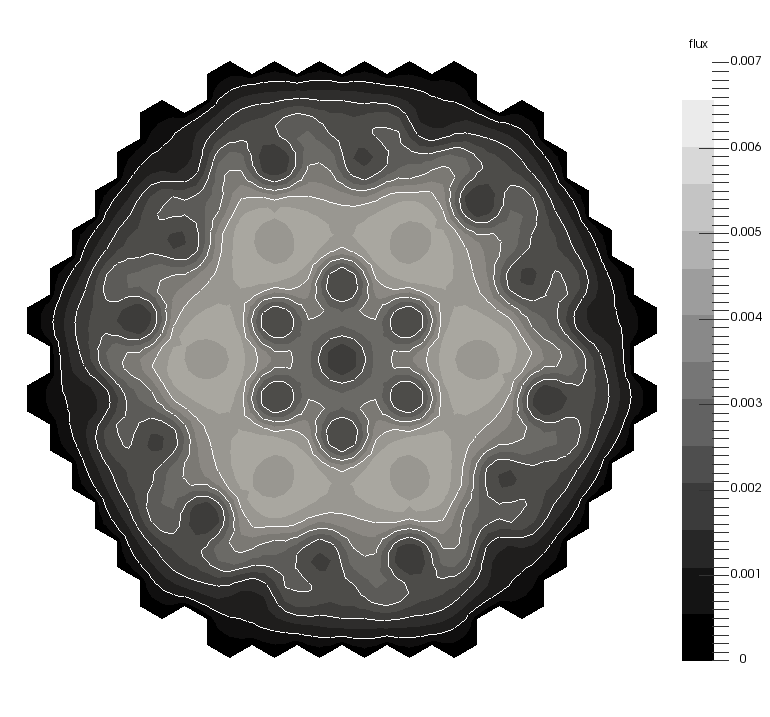
\includegraphics[width=0.9\linewidth]{14-4.png}  $t=0.005$} \\
\end{minipage}
\caption{Эволюция $\phi_2(t)$.}
\label{fig:14}
  \end{center}
\end{figure}

Приведем аналогичные расчетные данные по динамической задаче с учетом запаздывающих нейтронов, когда 
$T=1\cdot 10^{-2}$. Будем использовать шаги по времени $\tau = 1\cdot 10^{-4}, 2\cdot 10^{-4}, 4\cdot 10^{-4}, 8\cdot 10^{-4}$ в случае чисто неявной схемы и  $\tau=5\cdot 10^{-6}, 1\cdot 10^{-5},2\cdot 10^{-5}, 4\cdot 10^{-4}$ в случае явно-неявной схемы. Реперным решением ($ref$) в этой задаче будет решение при чисто неявной аппроксимации 
по времени с шагом $\tau = 5 \cdot 10^{-5}$.

Зависимости $\eta(t)$ и $\theta(t)$ от используемого шага по времени приведена на рис.\ref{fig:15} для чисто неявной схемы и на рис.\ref{fig:16} --- для явно-неявной схемы. Чисто неявная схема снова имеет существенно более высокую точность, чем явно-неявная схема.
Приведены также (рис.\ref{fig:17},\ref{fig:18}) отнормированые решения $\overline{\phi}_1$ и $\overline{\phi}_2$ на характерные моменты времени $t=0.0001, 0.0004, 0.0016$ и $0.0064$ секунд.

\begin{figure}[H]
  \begin{center}
\begin{minipage}{0.49\linewidth}
\center{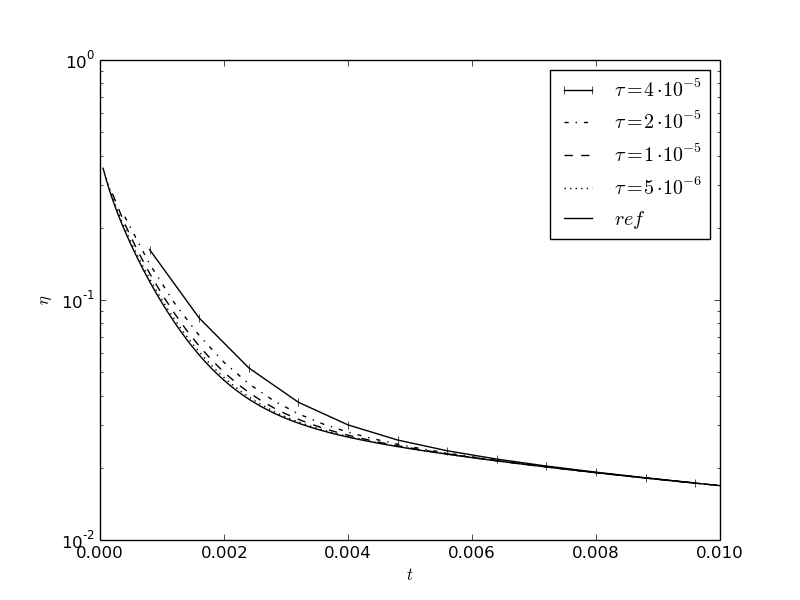
\includegraphics[width=1\linewidth]{15-1.png}} \\
\end{minipage}
\hfill
\begin{minipage}{0.49\linewidth}
\center{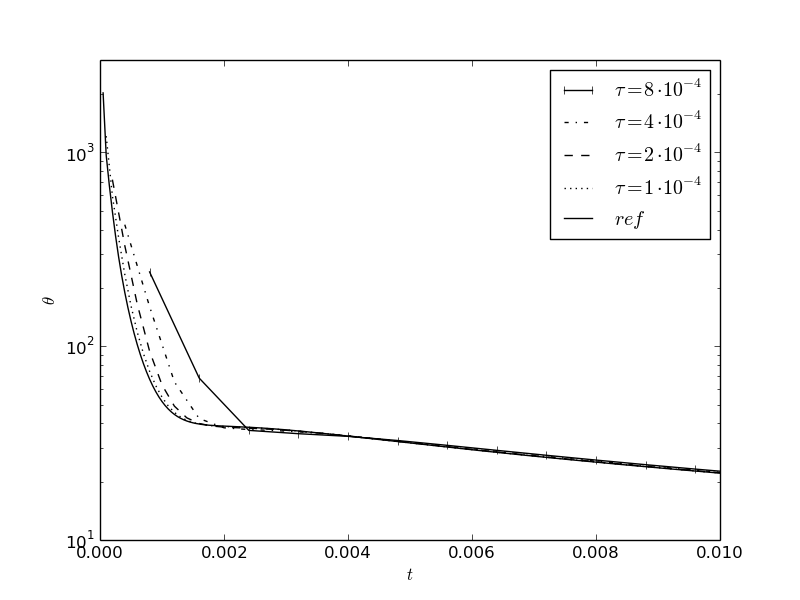
\includegraphics[width=1\linewidth]{15-2.png}} \\
\end{minipage}
\caption{Чисто неявная схема (\ref{17}).}
\label{fig:15}
  \end{center}
\end{figure}

\begin{figure}[H]
  \begin{center}
\begin{minipage}{0.49\linewidth}
\center{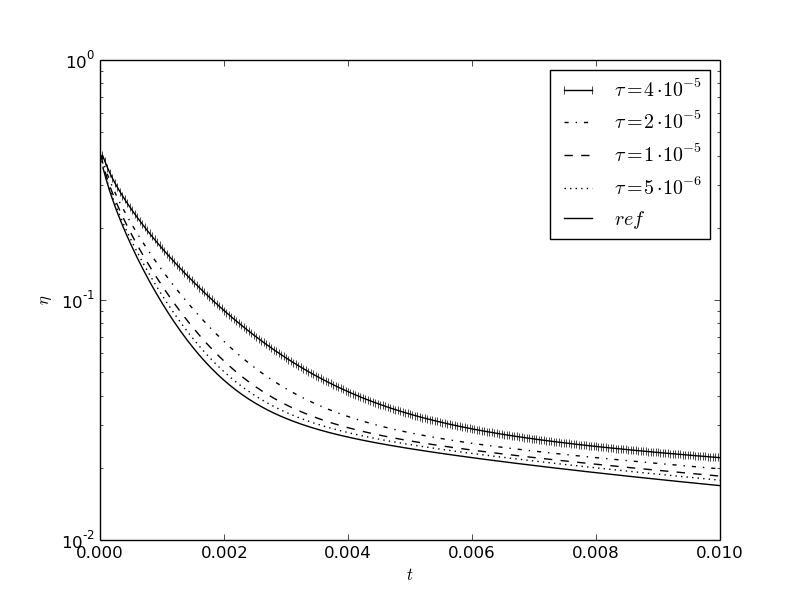
\includegraphics[width=1\linewidth]{16-1.png}} \\
\end{minipage}
\hfill
\begin{minipage}{0.49\linewidth}
\center{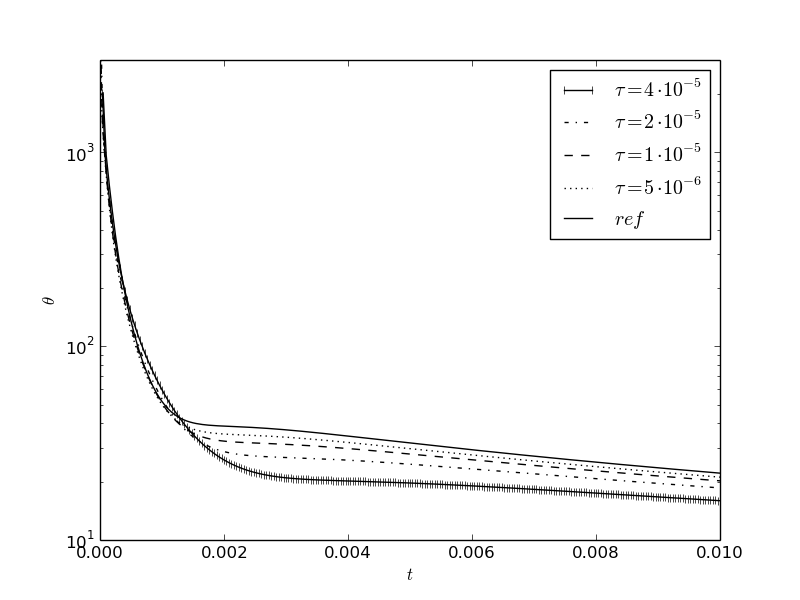
\includegraphics[width=1\linewidth]{16-2.png}} \\
\end{minipage}
\caption{Явно-неявная схема (\ref{18}).}
\label{fig:16}
  \end{center}
\end{figure}
 
\begin{figure}[H]
\begin{center}
\begin{minipage}{0.49\linewidth}
\center{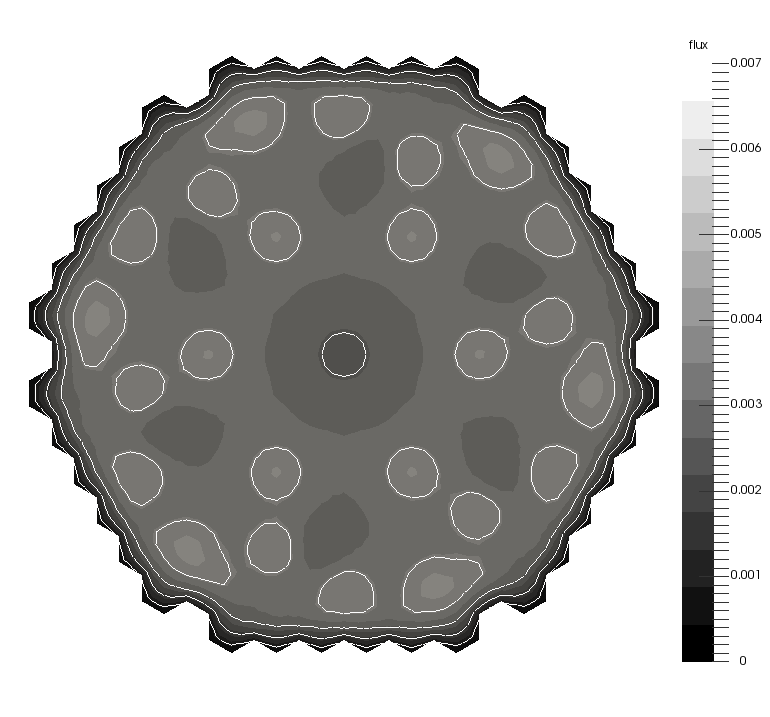
\includegraphics[width=0.9\linewidth]{17-1.png}  $t=0.0001$} \\
\end{minipage}
\hfill
\begin{minipage}{0.49\linewidth}
\center{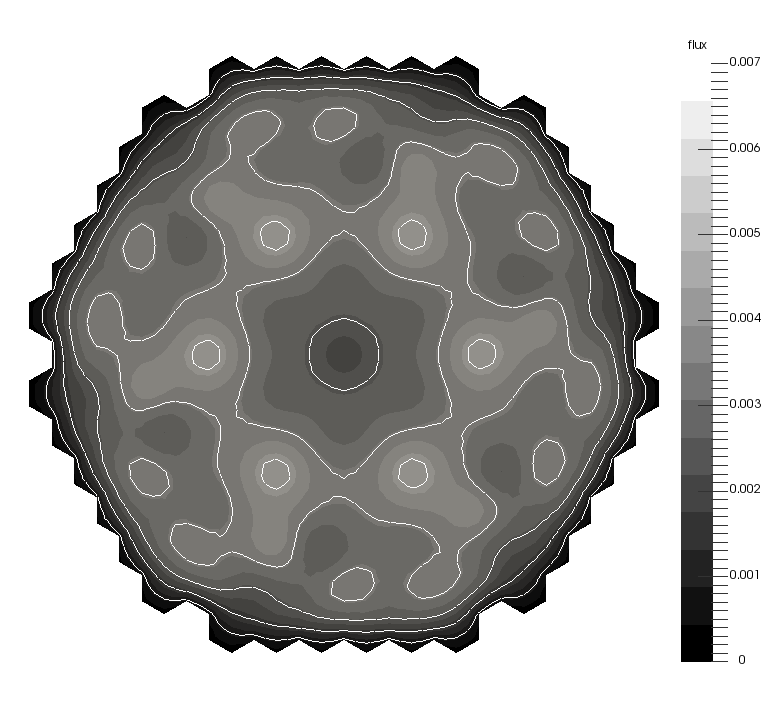
\includegraphics[width=0.9\linewidth]{17-2.png}  $t=0.0004$} \\
\end{minipage}
\hfill
\begin{minipage}{0.49\linewidth}
\center{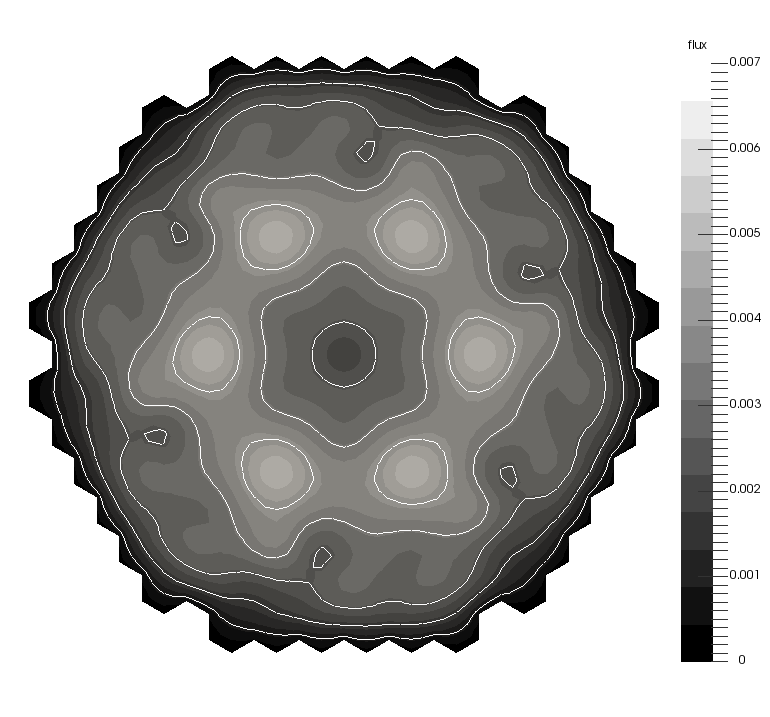
\includegraphics[width=0.9\linewidth]{17-3.png}  $t=0.0016$} \\
\end{minipage}
\hfill
\begin{minipage}{0.49\linewidth}
\center{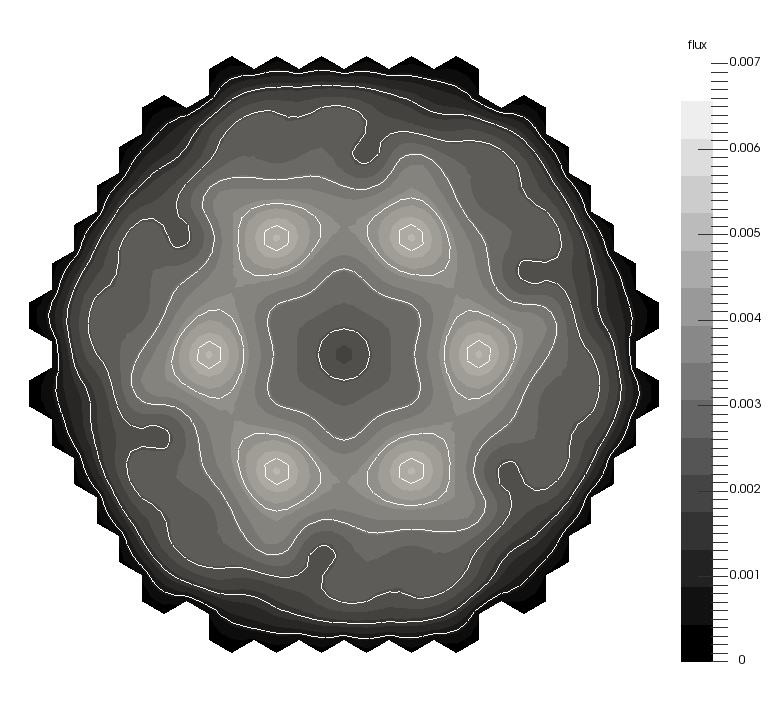
\includegraphics[width=0.9\linewidth]{17-4.png}  $t=0.0064$} \\
\end{minipage}
\caption{Эволюция $\phi_1(t)$.}
\label{fig:17}
  \end{center}
\end{figure}

\begin{figure}[H]
  \begin{center}
\begin{minipage}{0.49\linewidth}
\center{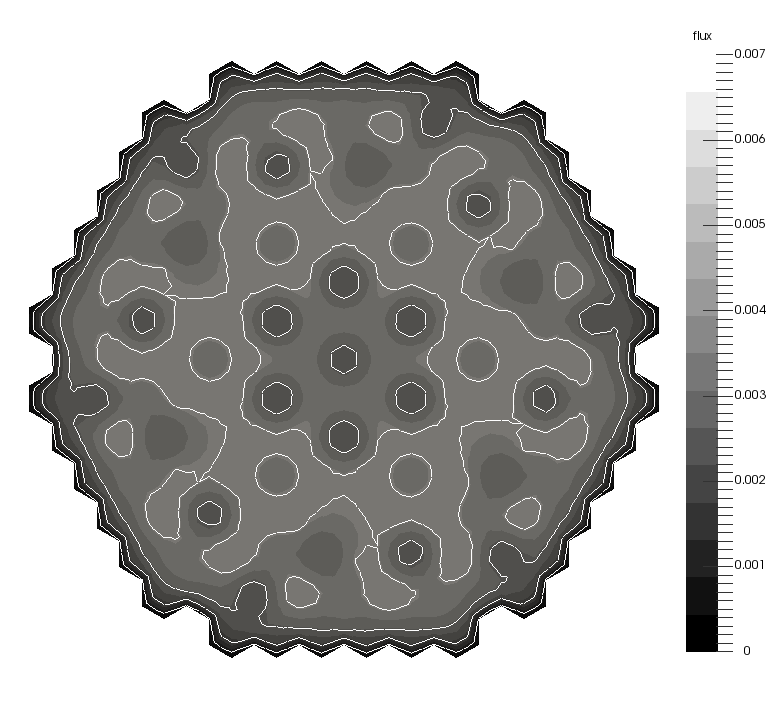
\includegraphics[width=1\linewidth]{18-1.png}  $t=0.0001$} \\
\end{minipage}
\hfill
\begin{minipage}{0.49\linewidth}
\center{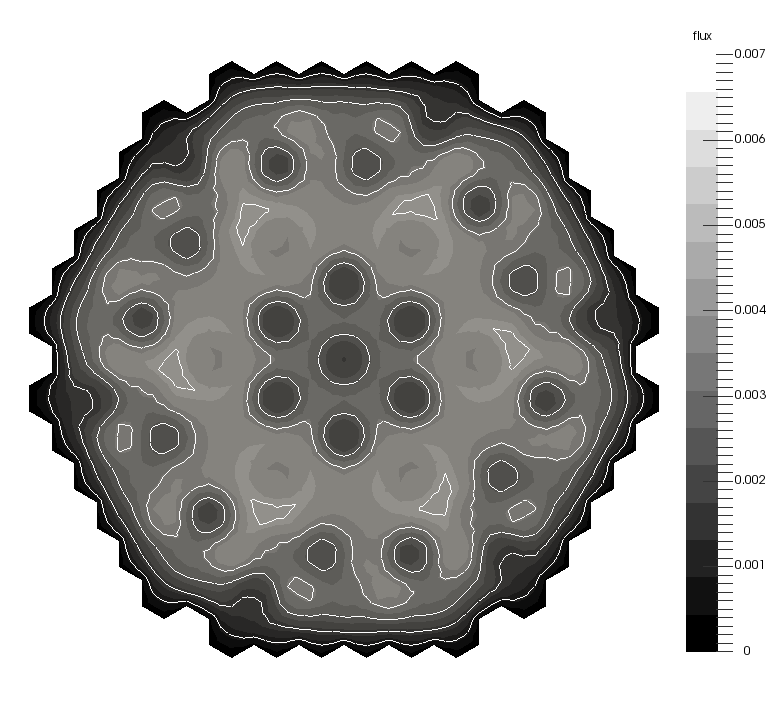
\includegraphics[width=1\linewidth]{18-2.png}  $t=0.0004$} \\
\end{minipage}
\hfill
\begin{minipage}{0.49\linewidth}
\center{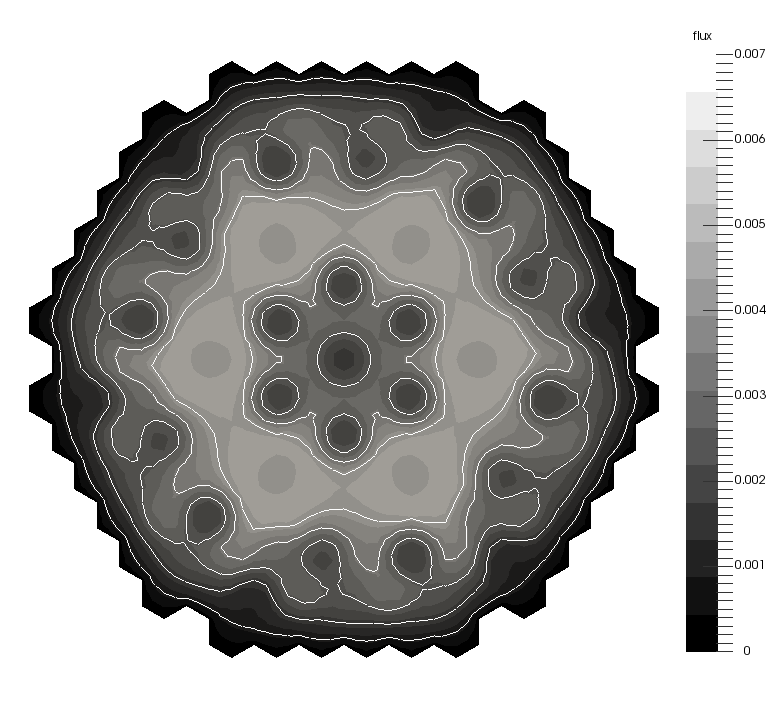
\includegraphics[width=1\linewidth]{18-3.png}  $t=0.0016$} \\
\end{minipage}
\hfill
\begin{minipage}{0.49\linewidth}
\center{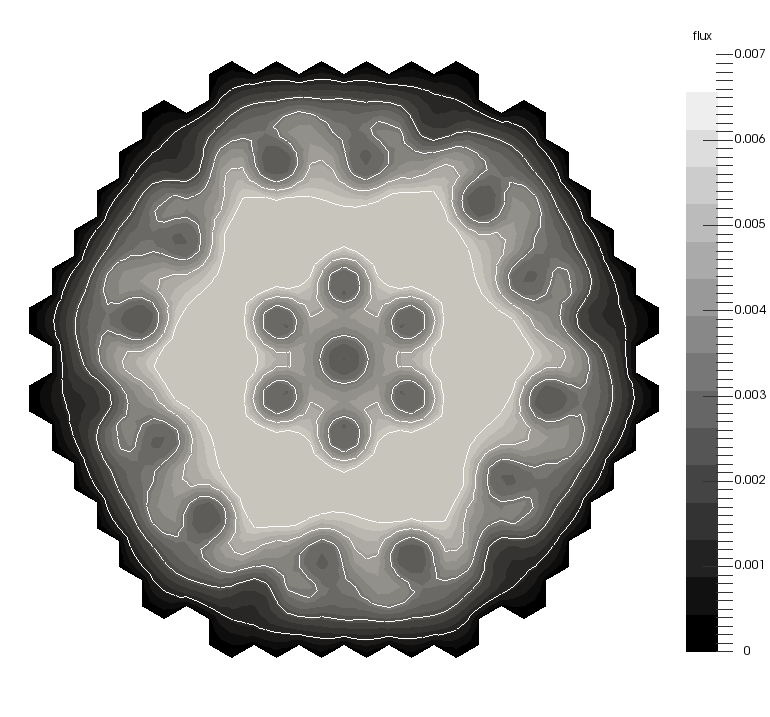
\includegraphics[width=1\linewidth]{18-4.png}  $t=0.0064$} \\
\end{minipage}
\caption{Эволюция $\overline{\phi}_2(t)$.}
\label{fig:18}
  \end{center}
\end{figure}


\section{Выводы}


Рассмотрена нестационарная задача диффузии нейтронов в ядерном реакторе 
при использовании многогруппового приближения. 
Выделена $\alpha$-спектральная задача, которая характеризует
динамическое нейтронное поле ядерного реактора  на асимптотической стадии при больших временах --- регулярный режим.

Вычислительный алгоритм приближенного решения спектральных задач базируется на стандартной конечно-элементной аппроксимации по пространству при использовании лагранжевых конечных элементов степени $p=1,2,3$. 
Матричная спектральная задача решается с использованием
свободной библиотеки SLEPc. 
Контроль точности приближенного решения проводиться на последовательности сгущающихся сеток с использованием конечных элементов различной степени.

Для приближенного решения нестационарной задачи использовались стандартная
чисто неявная схема первого порядка аппроксимации и симметричная
схема (схема Кранка-Николсон) второго порядка. 
Рассмотрена также явно-неявная схема, когда члены уравнения описывающие 
генерацию нейтронов беруться с нижнего временного слоя.
Такая схема более удобна в плане вычислительной реализации, чем стандартные схемы с весами.

Рассмотрена нестационарная задача диффузии нейтронов с выходом на регулярный режим в двух случаях: с учетом запаздывающих нейтронов и без учета запаздывающих нейтронов. 
Тестовые расчеты выполнены в двумерном приближении для ядерного реактора ВВВЭР-1000 без отражателя с использованием двухгруппового диффузионного приближения. Установлена хорошая отделимость собственных значений в $\alpha$-спектральной задаче с учетом и без учета запаздывающих нейтронов. 
Наблюдается хорошая сходимость нестационарной задачи при уменьшении шага по времени для чисто неявной схемы. Явно-неявная схема сходится намного хуже,  чем чисто неявная схема. Схема Кранка-Николсон хоть и имеет второй порядок аппроксимации, практически непригодна для моделирования регулярного режима ядерного реактора. 


%\bibliographystyle{gost705}
%\bibliography{mm_avvs}

\ifx\undefined\BibEmph\def\BibEmph#1{#1}\else\fi
\ifx\undefined\href\def\href#1#2{#2}\else\fi
\ifx\undefined\url\def\url#1{\texttt{#1}}\else\fi
\ifx\undefined\urlprefix\def\urlprefix{URL: }\else\fi
\ifx\undefined\BibUrl\def\BibUrl#1{\urlprefix\url{#1}}\else\fi
\ifx\undefined\BibUrlDate\long\def\BibUrlDate#1{({%
\cyr\cyrd\cyra\cyrt\cyra\ %
\cyro\cyrb\cyrr\cyra\cyrshch\cyre\cyrn\cyri\cyrya}: #1)}\else\fi
\ifx\undefined\BibAnnote\long\def\BibAnnote#1{#1}\else\fi
\begin{thebibliography}{10}
\def\selectlanguageifdefined#1{
\expandafter\ifx\csname date#1\endcsname\relax
\else\language\csname l@#1\endcsname\fi}

\bibitem{duderstadt1976nuclear}
\selectlanguageifdefined{english}
\BibEmph{Duderstadt~J.~J., Hamilton~L.~J.} Nuclear Reactor Analysis.
\newblock Wiley, 1976.

\bibitem{hetrick1971dynamics}
\selectlanguageifdefined{english}
\BibEmph{Hetrick~D.~L.} Dynamics of Nuclear Reactors.
\newblock University of Chicago Press, 1971.

\bibitem{stacey}
\selectlanguageifdefined{english}
\BibEmph{Stacey~W.~M.} Nuclear Reactor Physics.
\newblock Wiley, 2007.

\bibitem{marchuk1986numerical}
\selectlanguageifdefined{english}
\BibEmph{Marchuk~G.~I., Lebedev~V.~I.} Numerical Methods in the Theory of
  Neutron Transport.
\newblock Harwood Academic Pub., 1986.

\bibitem{lewis1993computational}
\selectlanguageifdefined{english}
\BibEmph{Lewis~E.~E., Miller~W.~F.} Computational Methods of Neutron Transport.
\newblock American Nuclear Society, 1993.

\bibitem{sutton1996diffusion}
\selectlanguageifdefined{english}
\BibEmph{Sutton~T.~M., Aviles~B.~N.} Diffusion theory methods for spatial
  kinetics calculations~// \BibEmph{Progress in Nuclear Energy}.
\newblock 1996.
\newblock Vol.~30, no.~2.
\newblock P.~119--182.

\bibitem{cho2005fundamentals}
\selectlanguageifdefined{english}
\BibEmph{Cho~N.~Z.} Fundamentals and recent developments of reactor physics
  methods~// \BibEmph{Nuclear Engineering and Technology}.
\newblock 2005.
\newblock Vol.~37, no.~1.
\newblock P.~25--78.

\bibitem{smith1979analytic}
\selectlanguageifdefined{english}
\BibEmph{Smith~K.~S.} An analytic nodal method for solving the two-group,
  multidimensional, static and transient neutron diffusion equations: Ph.\,D.
  thesis~/ Massachusetts Institute of Technology.
\newblock 1979.

\bibitem{lawrence1986progress}
\selectlanguageifdefined{english}
\BibEmph{Lawrence~R.~D.} Progress in nodal methods for the solution of the
  neutron diffusion and transport equations~// \BibEmph{Progress in Nuclear
  Energy}.
\newblock 1986.
\newblock Vol.~17, no.~3.
\newblock P.~271--301.

\bibitem{grossman2007nodal}
\selectlanguageifdefined{english}
\BibEmph{Grossman~L.~M., Hennart~J.-P.} Nodal diffusion methods for space-time
  neutron kinetics~// \BibEmph{Progress in Nuclear Energy}.
\newblock 2007.
\newblock Vol.~49, no.~3.
\newblock P.~181--216.

\bibitem{brenner}
\selectlanguageifdefined{english}
\BibEmph{Brenner~S.~C., Scott~R.} {The Mathematical Theory of Finite Element
  Methods}.
\newblock Springer, 2008.

\bibitem{quarteroni}
\selectlanguageifdefined{english}
\BibEmph{Quarteroni~A., Valli~A.} {Numerical Approximation of Partial
  Differential Equations}.
\newblock Springer, 2008.

\bibitem{HagemanYoung1981}
\selectlanguageifdefined{english}
\BibEmph{Hageman~L.~A., Young~D.~M.} Applied Iterative Methods.
\newblock New York: Academic Press, 1981.

\bibitem{Saad2003}
\selectlanguageifdefined{english}
\BibEmph{Saad~Y.} Iterative methods for sparse linear systems.
\newblock Society for Industrial Mathematics, 2003.

\bibitem{Ascher2008}
\selectlanguageifdefined{english}
\BibEmph{Ascher~U.~M.} Numerical Methods for Evolutionary Differential
  Equations.
\newblock Society for Industrial Mathematics, 2008.

\bibitem{LeVeque2007}
\selectlanguageifdefined{english}
\BibEmph{LeVeque~R.~J.} Finite Difference Methods for Ordinary and Partial
  Differential Equations. Steady-State and Time-Dependent Problems.
\newblock Society for Industrial Mathematics, 2007.

\bibitem{HundsdorferVerwer2003}
\selectlanguageifdefined{english}
\BibEmph{Hundsdorfer~W.~H., Verwer~J.~G.} Numerical Solution of Time-dependent
  Advection-diffusion-reaction Equations.
\newblock Springer Verlag, 2003.

\bibitem{Butcher2008}
\selectlanguageifdefined{english}
\BibEmph{Butcher~J.~C.} {Numerical Methods for Ordinary Differential
  Equations}.
\newblock Wiley, 2008.

\bibitem{HairerWanner2010}
\selectlanguageifdefined{english}
\BibEmph{Hairer~E., Wanner~G.} {Solving Ordinary Differential Equations II:
  Stiff and Differential-Algebraic Problems}.
\newblock Springer Verlag, 2010.

\bibitem{chou1990three}
\selectlanguageifdefined{english}
\BibEmph{Chou~H.~P., Lu~J.~R., Chang~M.~B.} A three-dimensional space-time
  model and its use in pressurized water reactor rod ejection analyses~//
  \BibEmph{Nuclear Technology}.
\newblock 1990.
\newblock Vol.~90, no.~2.
\newblock P.~142--154.

\bibitem{dahmani20013d}
\selectlanguageifdefined{english}
\BibEmph{Dahmani~M., Baudron~A.~M., Lautard~J.~J., Erradi~L.} A {3D} nodal
  mixed dual method for nuclear reactor kinetics with improved quasistatic
  model and a semi-implicit scheme to solve the precursor equations~//
  \BibEmph{Annals of Nuclear Energy}.
\newblock 2001.
\newblock Vol.~28, no.~8.
\newblock P.~805--824.

\bibitem{dodds1976accuracy}
\selectlanguageifdefined{english}
\BibEmph{Dodds~Jr~H.~L.} Accuracy of the quasistatic method for two-dimensional
  thermal reactor transients with feedback~// \BibEmph{Nuclear Science and
  Engineering}.
\newblock 1976.
\newblock Vol.~59, no.~3.
\newblock P.~271--276.

\bibitem{goluoglu2001time}
\selectlanguageifdefined{english}
\BibEmph{Goluoglu~S., Dodds~H.~L.} A time-dependent, three-dimensional neutron
  transport methodology~// \BibEmph{Nuclear Science and Engineering}.
\newblock 2001.
\newblock Vol. 139, no.~3.
\newblock P.~248--261.

\bibitem{Bell1970}
\selectlanguageifdefined{english}
\BibEmph{Bell~G.~I., Glasstone~S.} Nuclear Reactor Theory.
\newblock Van Nostrand Reinhold Company, 1970.

\bibitem{modak2007scheme}
\selectlanguageifdefined{english}
\BibEmph{Modak~R.~S., Gupta~A.} A scheme for the evaluation of dominant
  time-eigenvalues of a nuclear reactor~// \BibEmph{Annals of Nuclear Energy}.
\newblock 2007.
\newblock Vol.~34, no.~3.
\newblock P.~213--221.

\bibitem{verdu20103d}
\selectlanguageifdefined{english}
\BibEmph{Verdu~G., Ginestar~D., Roman~J., Vidal~V.} {3D} alpha modes of a
  nuclear power reactor~// \BibEmph{Journal of Nuclear Science and Technology}.
\newblock 2010.
\newblock Vol.~47, no.~5.
\newblock P.~501--514.

\bibitem{luikov2012analytical}
\selectlanguageifdefined{english}
\BibEmph{Luikov~A.} Analytical Heat Diffusion Theory.
\newblock Academic Press, 1968.

\bibitem{samarskii1996computational}
\selectlanguageifdefined{english}
\BibEmph{Samarskii~A.~A., Vabishchevich~P.~N.} Computational Heat Transfer.
\newblock Wiley, 1996.

\bibitem{Samarskiibook}
\selectlanguageifdefined{english}
\BibEmph{Samarskii~A.~A.} The Theory of Difference Schemes.
\newblock New York: Marcel Dekker, 2001.

\bibitem{SamarskiiGulin1973}
\selectlanguageifdefined{russian}
\BibEmph{Самарский~А.~А., Гулин~А.~В.} Устойчивость
  разностных схем.
\newblock Москва: Наука, 1973.

\bibitem{Gear1971}
\selectlanguageifdefined{english}
\BibEmph{Gear~C.~W.} {Numerical Initial Value Problems in Ordinary Differential
  Equations}.
\newblock NJ: Prentice Hall, 1971.

\bibitem{fenics}
\selectlanguageifdefined{english}
\BibEmph{Logg~A., Mardal~K.~A., Wells~G.} Automated Solution of Differential
  Equations by the Finite Element Method: The FEniCS Book.
\newblock Springer, 2012.

\bibitem{slepc}
\selectlanguageifdefined{english}
\BibEmph{Campos~C., Roman~J., Romero~E., Tomas~A.}
\newblock SLEPc Users Manual, 2013.

\bibitem{chao}
\selectlanguageifdefined{english}
\BibEmph{Chao~Y.~A., Shatilla~Y.~A.} Conformal mapping and hexagonal nodal
  methods-{II}: Implementation in the {ANC-H Code}.~// \BibEmph{Nuclear Science
  and Engineering}.
\newblock 1995.
\newblock Vol. 121.
\newblock P.~210--225.

\end{thebibliography}



\end{document}
